% Options for packages loaded elsewhere
\PassOptionsToPackage{unicode}{hyperref}
\PassOptionsToPackage{hyphens}{url}
%
\documentclass[
  10pt,
]{book}
\usepackage{amsmath,amssymb}
\usepackage{lmodern}
\usepackage{iftex}
\ifPDFTeX
  \usepackage[T1]{fontenc}
  \usepackage[utf8]{inputenc}
  \usepackage{textcomp} % provide euro and other symbols
\else % if luatex or xetex
  \usepackage{unicode-math}
  \defaultfontfeatures{Scale=MatchLowercase}
  \defaultfontfeatures[\rmfamily]{Ligatures=TeX,Scale=1}
\fi
% Use upquote if available, for straight quotes in verbatim environments
\IfFileExists{upquote.sty}{\usepackage{upquote}}{}
\IfFileExists{microtype.sty}{% use microtype if available
  \usepackage[]{microtype}
  \UseMicrotypeSet[protrusion]{basicmath} % disable protrusion for tt fonts
}{}
\makeatletter
\@ifundefined{KOMAClassName}{% if non-KOMA class
  \IfFileExists{parskip.sty}{%
    \usepackage{parskip}
  }{% else
    \setlength{\parindent}{0pt}
    \setlength{\parskip}{6pt plus 2pt minus 1pt}}
}{% if KOMA class
  \KOMAoptions{parskip=half}}
\makeatother
\usepackage{xcolor}
\IfFileExists{xurl.sty}{\usepackage{xurl}}{} % add URL line breaks if available
\IfFileExists{bookmark.sty}{\usepackage{bookmark}}{\usepackage{hyperref}}
\hypersetup{
  pdftitle={Jamaica's Preparedness ~Diagnosis},
  pdfauthor={CARICOM},
  hidelinks,
  pdfcreator={LaTeX via pandoc}}
\urlstyle{same} % disable monospaced font for URLs
\usepackage{longtable,booktabs,array}
\usepackage{calc} % for calculating minipage widths
% Correct order of tables after \paragraph or \subparagraph
\usepackage{etoolbox}
\makeatletter
\patchcmd\longtable{\par}{\if@noskipsec\mbox{}\fi\par}{}{}
\makeatother
% Allow footnotes in longtable head/foot
\IfFileExists{footnotehyper.sty}{\usepackage{footnotehyper}}{\usepackage{footnote}}
\makesavenoteenv{longtable}
\usepackage{graphicx}
\makeatletter
\def\maxwidth{\ifdim\Gin@nat@width>\linewidth\linewidth\else\Gin@nat@width\fi}
\def\maxheight{\ifdim\Gin@nat@height>\textheight\textheight\else\Gin@nat@height\fi}
\makeatother
% Scale images if necessary, so that they will not overflow the page
% margins by default, and it is still possible to overwrite the defaults
% using explicit options in \includegraphics[width, height, ...]{}
\setkeys{Gin}{width=\maxwidth,height=\maxheight,keepaspectratio}
% Set default figure placement to htbp
\makeatletter
\def\fps@figure{htbp}
\makeatother
\setlength{\emergencystretch}{3em} % prevent overfull lines
\providecommand{\tightlist}{%
  \setlength{\itemsep}{0pt}\setlength{\parskip}{0pt}}
\setcounter{secnumdepth}{5}
\usepackage{booktabs}
\usepackage{booktabs}
\usepackage{longtable}
\usepackage{array}
\usepackage{multirow}
\usepackage{wrapfig}
\usepackage{float}
\usepackage{colortbl}
\usepackage{pdflscape}
\usepackage{tabu}
\usepackage{threeparttable}
\usepackage{threeparttablex}
\usepackage[normalem]{ulem}
\usepackage{makecell}
\usepackage{xcolor}
\ifLuaTeX
  \usepackage{selnolig}  % disable illegal ligatures
\fi
\usepackage[]{natbib}
\bibliographystyle{plainnat}

\title{Jamaica's Preparedness ~Diagnosis}
\author{CARICOM}
\date{2022-06-20}

\begin{document}
\maketitle

{
\setcounter{tocdepth}{1}
\tableofcontents
}
\hypertarget{welcome}{%
\chapter*{Welcome}\label{welcome}}
\addcontentsline{toc}{chapter}{Welcome}

This is the website for Jamaica's Preparedness Diagnosis Report by GEI and CLEAR LAC!

\hypertarget{part-preface}{%
\part{Preface}\label{part-preface}}

\hypertarget{acknowledgements}{%
\chapter*{Acknowledgements}\label{acknowledgements}}
\addcontentsline{toc}{chapter}{Acknowledgements}

The CLEAR LAC team wishes to thank everyone involved in preparing this document. Especially to:

\begin{itemize}
\item
  Dr.~Kyra Paul, Dominica´s Executive Coordinator for the Collaboration on RBM.
\item
  Mrs.~Leah St.~Jean, Dominica's Junior Executive Coordinator for the Collaboration on RBM.
\item
  Mrs.~Maurya West-Myers and Mr.~Leonardo Lemes from the Global Evaluation Initiative
\item
  Mrs.~Hipolina Joseph and Ms.~Stacy-Ann Barnes, from the CARICOM Secretariat
\item
  The team of the CLEAR LAC´s interns who supported in the process of preparing this diagnosis: Alexia Galarza, Carolina Zepeda, Gisela Hurtado, Mariana Espinoza, Emilio Olmos and Lothar Rojas.
\end{itemize}

\hypertarget{acronyms-and-abbreviations}{%
\chapter*{Acronyms and abbreviations}\label{acronyms-and-abbreviations}}
\addcontentsline{toc}{chapter}{Acronyms and abbreviations}

\textbf{CARICOM} -The Caribbean Community

\textbf{CLEAR LAC} - Center for Learning on Evaluation and Results for Latin America and Caribbean

\textbf{EPMS} -- Employee Performance Management System

\textbf{EPMP} -- Employee Performance Management Policy

\textbf{FAAA} -- Financial Administration and Audit Act

\textbf{GEI} -- Global Evaluation Initiative

\textbf{GoJ} -- Government of Jamaica

\textbf{MDAs} -- Ministries, Departments and Agencies

\textbf{MIND} -- Management Institute for National Development MOFPS -Ministry of Finance and the Public Service

\textbf{MTF} - Mid-Term Socio-Economic Policy Framework

\textbf{MTRBB} -- Medium-Term Results Based Budgeting

\hypertarget{list-of-figures-and-tables}{%
\chapter*{List of figures and tables}\label{list-of-figures-and-tables}}
\addcontentsline{toc}{chapter}{List of figures and tables}

\textbf{Figure 1.} Theory of Change

\textbf{Figure 2.} Dimensions of an ideal RBM system

\textbf{Figure 3.} Working Process defined for the CARICOM Collaboration

\textbf{Figure 4.} Stages of the Preparedness Diagnostic

\textbf{Figure 5.} Level of progress of the Ideal RBM System

\textbf{Figure 6.} From an ideal RBM system to the roadmaps

\textbf{Figure 7.} Learning loop

\textbf{Figure 8.} How to identify the current level of the RBM system maturity

\textbf{Table 1.} Jamaica's Preparedness Diagnostic Numbers

\textbf{Table 2.} General Statistics of Jamaica

\textbf{Table 3.} Stakeholders Analysis

\textbf{Table 4:} Elements and sub-elements of the Ideal RBM System

\textbf{Table 5:} Detailed results of the Preparedness Diagnostic for Jamaica

\textbf{Table 6.} List of participants in the Preparedness Diagnostic

\hypertarget{definitions-and-concepts}{%
\chapter*{Definitions and concepts}\label{definitions-and-concepts}}
\addcontentsline{toc}{chapter}{Definitions and concepts}

\textbf{Evaluation} - The systematic and objective assessment of an ongoing or completed project, programme, or policy, including its design, implementation, and results.

\textbf{Monitoring} -- The continuous and systematic collection of data on specified indicators, to provide information on the extent to which resources have been used and what outputs have been achieved or produced.

\textbf{Result} - Clearly defined and demonstrable output, outcome, or impact (intended or unintended, positive and/or negative) of an intervention.

\textbf{Results-Based Management System (RBM System)}\footnote{This concept was developed following internationally recognised standards and approaches and contextualised to the particular case of CARICOM} - It is a global and systemic approach to management that orients all strategies, actions, and resources (both human and material) towards improving decision-making and the achievement and measurement of clearly defined and demonstrable results expected by governments and institutions, whether national, regional, or global.

This systemic approach can be analysed at three levels (considering all the relationships that may exist between them) for CARICOM: the national level, the regional institutions level, and the whole-regional / CARICOM level. These levels are individual and do not have a defined hierarchy, as they have their own institutional, human, financial and multidimensional contextual characteristics that make them independent of each other. Nevertheless, the articulation between them is relevant to understanding how RBM operates in the region.

The RBM system can, in turn, be composed of different sub-systems (that are systems by themselves). Some of the most important, but not the only ones, are: the monitoring and evaluation (M\&E) sub-system (with the formal document that institutionalises it: the M\&E Policy or Framework, if it exists); the data and information sub-system, which generates, processes, systematises and publishes relevant information to know and scale the multidimensional situation of the country or institution and thus identify problems to be addressed and guide decision-making; the human resources management sub-system, which builds and constantly strengthens the necessary capacities to have the staff with the capabilities to carry out the M\&E and RBM activities necessary to achieve and measure the expected results, etc.

RBM policies, on the other hand, are key elements of a sustainable RBM system but are not, by themselves, the system. RBM policies are the normative framework that: defines how the RBM system will be structured; establishes the guiding principles for the results-oriented approach; communicates what RBM entails for the country, institution or region; identifies stakeholders to be involved and their responsibilities; and identifies the needs to execute the necessary activities, among other elements. National, institutional, and regional RBM systems linkages may be established in RBM policies, which may have shared elements.

In this way, we should not confuse the RBM system with technological applications, platforms, software, or digital repositories with data or information contained and systematised, with the other sub-systems (described above) that conforms it, or with the RBM policies; but we should assume that to have a fully operational RBM system, it is necessary to seek a good articulation between all the sub-systems and levels, so we can achieve and measure the expected results, both at the national and regional levels.

\hypertarget{part-preparedness-diagnosis}{%
\part{Preparedness Diagnosis}\label{part-preparedness-diagnosis}}

\hypertarget{introduction}{%
\chapter{Introduction}\label{introduction}}

In July 2014, the Conference of Heads of Government of the Caribbean Community (CARICOM), approved the CARICOM Strategic Plan 2015-2019 which articulated the need for a more results-focused approach to programme and project management, and committed the Caribbean Community Secretariat to establish a planning, monitoring and evaluation (M\&E), and reporting system based on the principles of Results-Based Management (RBM). In executing the tenets of the Community Strategic Plan, all implementing partners have expressed concern about an \emph{implementation deficit}. This has resulted in poor implementation of public policy and Regional Public Goods in many Member States, culminating in low rates of successful program and project implementation across the Community.

Efforts to address the \emph{implementation deficit}, to promote a more results-focused approach to programme and project management, and to strengthen RBM in the Community commenced in 2016 with the engagement of the consulting firm Baastel, to develop the CARICOM RBM System and support its institutionalisation at the CARICOM Secretariat. In October 2019, the CARICOM Secretariat requested technical assistance\footnote{With non-lending Technical Assistance (TA) the Bank helps clients to implement reform and/or strengthen institutions. Qualified TA activity must meet the following criteria: have a primary intent of enabling an external client to implement reform and/or strengthen institutions; be linked to a Bank unit with clear accountability for the service provided.} from the World Bank's Independent Evaluation Group (IEG) to continue these efforts by supporting CARICOM in strengthening a result-oriented culture across the Community, which includes three implementing partners, the Member States, Regional Institutions, and the CARICOM Secretariat.

As part of the collaboration, the IEG and CLEAR LAC under the Global Evaluation Initiative (GEI) agreed to provide technical assistance in the establishment and institutionalisation of RBM policies, in addition to the Secretariat, to three pilot Member States (Dominica, Jamaica, and Saint Lucia) and three pilot Regional Institutions (the Caribbean Development Fund, the Caribbean Examinations Council, and the CARICOM Implementation Agency for Crime and Security). These pilots will serve as champions to support capacity strengthening in the remaining Member States and Regional Institutions, in collaboration with IEG and the CARICOM Secretariat.

In order to establish a customize roadmap to strengthen the pilot´s RBM Systems, a Preparedness Diagnostic was identified as a first step of the collaboration to assess the level of maturity of the systems and identify specific contextual and organizational features and milestones to be achieved over a over a five-year period.

This report presents the findings from the Preparedness Diagnostic for Jamaica. The report provides information on the existing strengthens and opportunities to develop a sustainable RBM System in the Member State.

The report consists of six sections, including the introduction. \protect\hyperlink{section2}{Section 2} will present Jamaica'sposition on the results of the Preparedness Diagnostic. \protect\hyperlink{section3}{Section 3} presents the methodology (including the Theory of Change of this activity); the Preparedness Diagnostic stages; and the ``Ideal RBM System,'' which consists of a four-dimension benchmark for this assessment).

\protect\hyperlink{section4}{Section 4} contains general and contextual information about Jamaica. This section also addresses the interest, expectations and challenges that may arise through the implementation of an RBM system using a whole of government approach. Additionally progress on the development of their RBM system based on the four dimensions is presented under this section.

\protect\hyperlink{section5}{Section 5} presents the main findings highlighting the level of progress for Jamaica in each of the four dimensions, and a stakeholder's analysis. Finally, \protect\hyperlink{sectionux5cux26}{Section 6} introduces the process for building a contextualized roadmap for advancing a sustainable RBM system for Jamaica, as well as a stakeholders' contribution analysis.

After reading this report, the reader will obtain a clear idea of the existing practices and elements to strength on and advance towards achieving a sustainable RBM system based on key elements. The report may also be used to guide discussions among relevant stakeholders to support sensitization of key stakeholders in the area of RBM practices; to share best practices with other Member States; as well as to promote existing promising practices that are being implemented.

Specifically, within the framework of this collaboration, the report represents the main input for the development of the contextualized medium-term roadmaps which will be facilitated through participatory workshops and engagements.

\hypertarget{section2}{%
\chapter{Jamaica's position on the Preparedness Diagnostic}\label{section2}}

{ Once the final report has been finalised including the development of the roadmaps, this section will present a position from the Member State (coordinated by the Executive Coordinator for this collaboration) on the process of the preparedness diagnostic, the main findings identified, and the role of the CLEAR LAC team and the CARICOM Secretariat while developing it. }

\hypertarget{section3}{%
\chapter{Methodology}\label{section3}}

This section presents the methodology and approach of the preparedness diagnostic used under this collaboration to strengthen RBM in the Community. It also presents the strengths and limitations of the methodology that should be considered when analysing the results or future replication exercises.

\hypertarget{theory-of-change-of-a-sustainable-rbm-system}{%
\section{Theory of Change of a sustainable RBM System}\label{theory-of-change-of-a-sustainable-rbm-system}}

The collaboration addresses an implementation deficit of public policies of CARICOM Member States that results in poor resolution of socio-economic problems which affects the well-being of the citizens..

The diagram below shows a summarized theory of change of the collaborations' activity. As described in previous sections, this report is intended to communicate the findings of a thorough RBM preparedness diagnostic which was conducted with Jamaica. The four stages of the preparedness diagnostic provided relevant information that served as inputs for this report. In addition, it provided a contextual framework, to identify a network of champions to support the process. These additional gains will inform the next steps required to develop the Jamaican RBM roadmap

This final report is the main input for the participatory workshops, for which specific processes have been defined and are presented in \protect\hyperlink{section5}{section 5}.The workshops will lead to the development of a contextualized roadmap with activities and responsibilities to advance the implementation of a sustainable RBM system, aligned to the four dimensions: \emph{Institutionalization, Operational Framework, Technical Capacity, and the Use of Evidence}. These dimensions are further described in the following subsection and \protect\hyperlink{appendixA}{Appendix A}.

The fulfilment and continuity of the activities integrating the roadmap, together with the continuous promotion and support of an enabling environment and a system of incentives with a whole of government/institution approach are:

\begin{itemize}
\item
  expected to lead to the institutionalisation of the RBM system (understood as the existence, acknowledgement, and communication of clear rules);
\item
  to the development of technical elements to support the system (understood as having developed capacity for generating and using the evidence that feeds the system);
\item
  to having an organizational design and actual roll-out of the system (understood as having structures and processes designed and implemented for generating evidence and enabling the fulfilment of the normative framework);
\item
  and finally, to a communication and persuasion strategy (understood as having timely access to evidence and knowing the paths to promote and measure its use).
\end{itemize}

\begin{center}\rule{0.5\linewidth}{0.5pt}\end{center}

\begin{figure}

{\centering 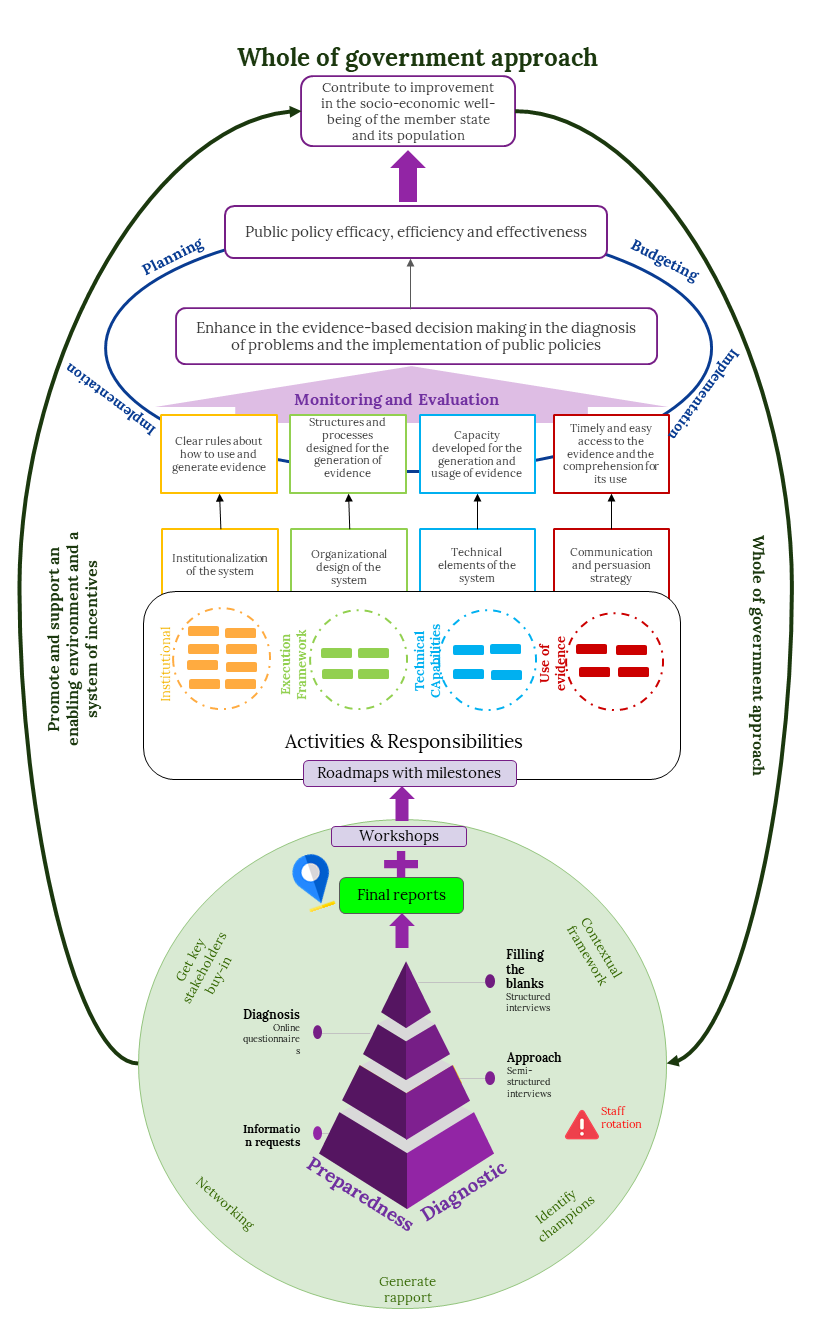
\includegraphics[width=0.75\linewidth]{./images/figure_1} 

}

\caption{Theory of Change}\label{fig:figure1}
\end{figure}

\begin{center}\rule{0.5\linewidth}{0.5pt}\end{center}

As these four dimensions advance and become solid practices, beyond compliance, the system moves towards an increase in evidence-based decision making across government/the institution and across planning, budgeting, and implementation that makes it possible to increase public policies' efficiency, efficacy, and effectiveness.

As the system stays in place and becomes mature, all the dimensions will be strengthened, the enabling environment will advance towards an RBM culture, and all of these will end up contributing to improve the socio-economic well-being of the member state and its population.

\hypertarget{ideal-rbm-system-and-working-process}{%
\section{Ideal RBM system and working process}\label{ideal-rbm-system-and-working-process}}

The development of an RBM System is a complex and nonlinear process that must be contextualized to the specific Member State. To establish a roadmap to strengthen or build an RBM system, the following three elements were considered:

\begin{enumerate}
\def\labelenumi{\arabic{enumi}.}
\tightlist
\item
  A benchmark against which to assess the level of maturity dubbed as ``Ideal RBM System''
\item
  A methodology to obtain general and specific recommendations and,
\item
  A working process and approach to generate ownership
\end{enumerate}

To establish the Ideal RBM system, multiple efforts done over time allow us to learn from experiences in different settings and identify good practices. These good practices represented useful inputs to determine ideal features of an RBM System. The CLEAR LAC team engaged in this collaboration defined four dimensions of an ideal sustainable RBM system (see \protect\hyperlink{fig:figure2}{Figure 2}):

\begin{center}\rule{0.5\linewidth}{0.5pt}\end{center}

\begin{figure}

{\centering 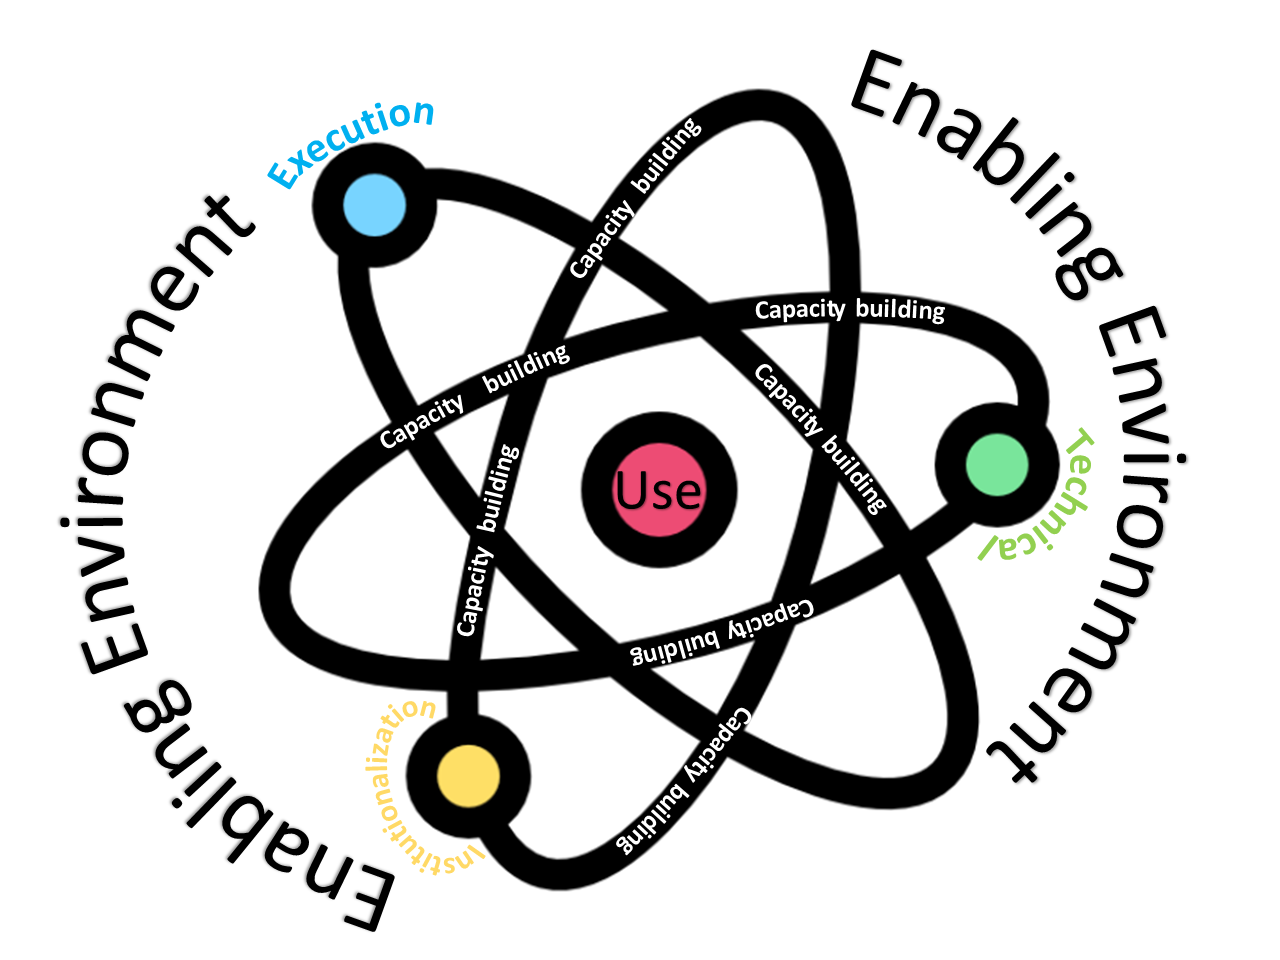
\includegraphics[width=1\linewidth]{./images/figure_2} 

}

\caption{Dimensions of an ideal RBM system}\label{fig:figure2}
\end{figure}

\begin{center}\rule{0.5\linewidth}{0.5pt}\end{center}

\begin{itemize}
\item
  \emph{Institutionalisation:} this dimension focuses on the formal rules that outline the RBM policy in the countries or regional institutions.
\item
  \emph{Execution framework:} this dimension focuses on the systems, resources, processes, methodologies, and tools necessary for the implementation of an RBM system, as well as on the enabling environment.
\item
  \emph{Technical capabilities:} this dimension focuses on the necessary capacities and abilities to implement an RBM System.
\item
  \emph{Use of evidence:} this dimension focuses on the dissemination strategies and incentives aimed at stakeholders with the purpose that they use the evidence generated by the RBM System.
\end{itemize}

Each dimension is integrated by key elements that constitute specific documents, normative frameworks, activities, incentives, among others. These different elements facilitate the operationalisation of the dimension as part of an RBM System. In a third level (beneath dimensions and elements), each element has sub-elements that list their ideal characteristics.

Once all the required information is gathered and analysed (based on the dimension-element-subelement structure) the dimensions will be assessed using a 3-level scale for each sub-element (no, yes, need of improvement)\footnote{For more details on the 3-level scale see \protect\hyperlink{appendixC}{appendix C}} .

For this last step, the progress rate in each sub-element within the element is added end and a cumulative value will be generated to rate the element. Subsequently, all the element values within each dimension are added to determine the progress rate of each dimension.

Finally, the average from the progress of the four dimensions will place each Member State at a specific level of progress (Early initiatives; Committed development; Growing RBM system; Consolidated practices, or Mature state) in the development and implementation of an RBM System (see \protect\hyperlink{appendixC}{Appendix C} for more details).

The working process, defined for this collaboration, identifies Monitoring and Evaluation (M\&E) activities as central elements to be developed and applied in order to affect planning, budgeting, and implementation. \protect\hyperlink{fig:figure3}{Figure 3} presents the working process and highlights the importance of evidence-based decision making (guided and made feasible by M\&E activities and supported, strengthened, and made sustainable through learning and accountability).

\begin{center}\rule{0.5\linewidth}{0.5pt}\end{center}

\begin{figure}

{\centering 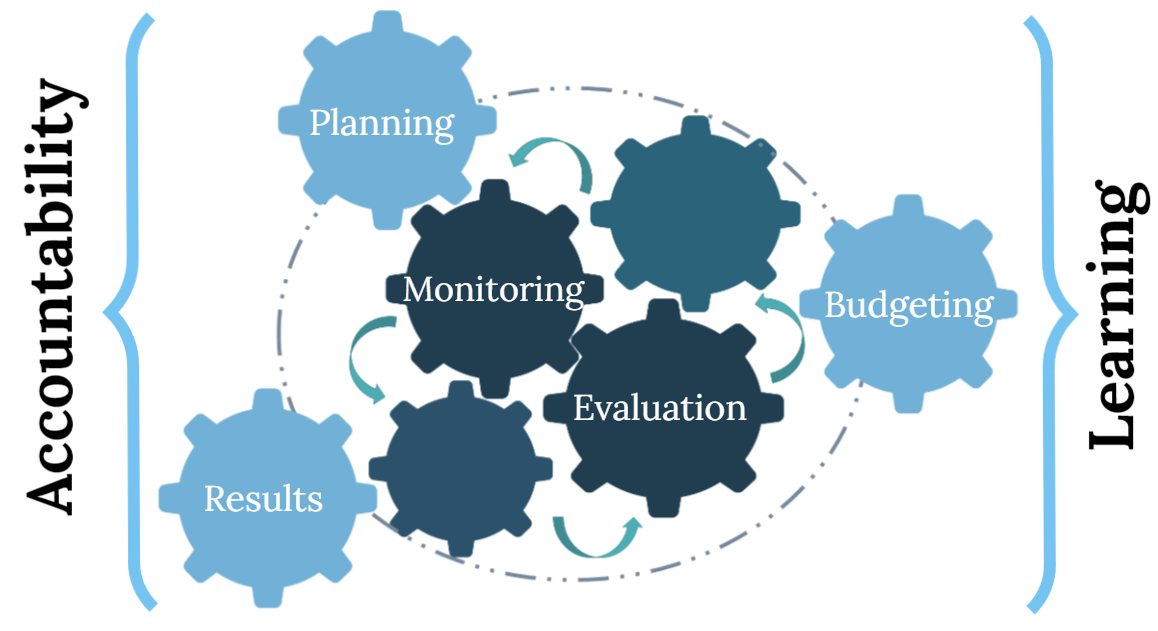
\includegraphics[width=1\linewidth]{./images/figure_3} 

}

\caption{Working Process defined for the CARICOM Collaboration}\label{fig:figure3}
\end{figure}

\begin{center}\rule{0.5\linewidth}{0.5pt}\end{center}

One significant component to strengthen RBM in the Community is to build, in a participatory process, specific roadmaps to continue the development of RBM Systems for each pilot member state and regional institution. The member states and regional institutions participating in the pilot have relevant but heterogeneous advances achieving this goal. To identify these advances, guide the analysis of the Preparedness Diagnostic stages, and develop ownership, the roadmap will be defined in workshops with key stakeholders involved in different levels (management, coordination, and operation).

\hypertarget{stages-of-the-preparedness-diagnostic}{%
\section{Stages of the Preparedness Diagnostic}\label{stages-of-the-preparedness-diagnostic}}

The Preparedness Diagnostic (PD) is a four-stage methodology designed to gain a deep understanding of the characteristics of the Member State to inform the development of an RBM System. One main assumption underpinning the methodological design of the PD, is that building a sustainable RBM System requires the active involvement of multiple stakeholders. The PD uses different data collection methods to identify and engage these stakeholders at different stages as well as to obtain information to understand the current policy environment; stakeholder's interests, their roles, motivations, relationship dynamics; map existing institutional structures, practices, and mechanisms; and define capacity building needs.

To successfully execute the PD, the CLEAR LAC team, in collaboration with the CARICOM Secretariat, selected Executive Coordinators who are representatives for the collaboration from the three Member States (Dominica, Jamaica and Saint Lucia) and the three Regional Institutions (the CARICOM Development Fund, the Caribbean Examinations Council and the CARICOM Implementation Agency for Crime and Security). The role of the Executive Coordinators was key to execute the PD as they have an overall knowledge of their Member State or Regional Institution and have experience in RBM. As Executive Coordinators and key informants, they acted as focal points and contributed to identifying and engaging relevant stakeholders at the different stages of the PD.

\hypertarget{stages-of-the-pd}{%
\subsection*{Stages of the PD}\label{stages-of-the-pd}}
\addcontentsline{toc}{subsection}{Stages of the PD}

The four stages of the PD (presented in \protect\hyperlink{fig:figure4}{Figure 4} ) are implemented according to a specific sequence and were customized based on the findings of the previous stage. They also involve the participation of different stakeholders to obtain a broad perspective of the pilot Member States and Regional Institutions. The figure below provides a brief description of the approach for implementing the stages.

\begin{center}\rule{0.5\linewidth}{0.5pt}\end{center}

\begin{figure}

{\centering 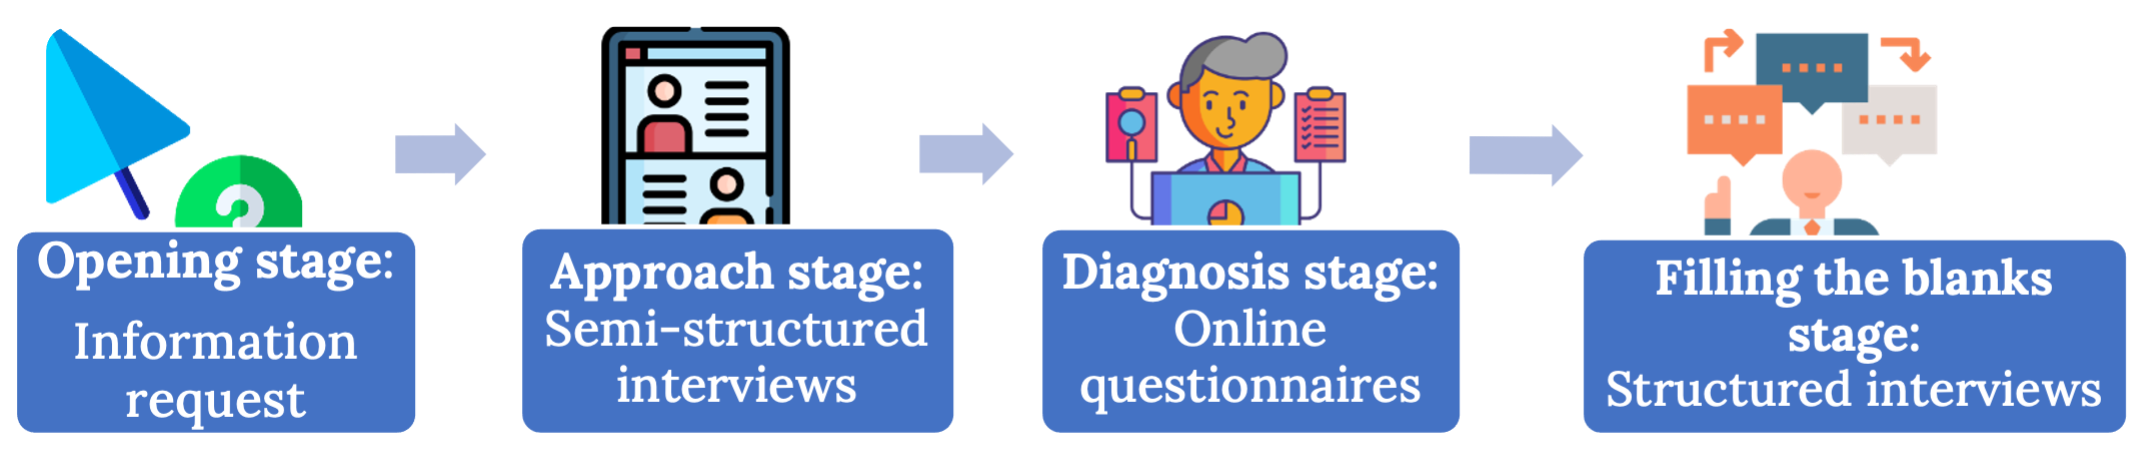
\includegraphics[width=1\linewidth]{./images/figure_4} 

}

\caption{Stages of the Preparedness Diagnostic}\label{fig:figure4}
\end{figure}

\begin{center}\rule{0.5\linewidth}{0.5pt}\end{center}

The \textbf{Opening stage} consisted of a request for different documents from the Executive Coordinators, regarding the pilots' planning, budgeting, and M\&E practices. The desk review and analysis of these documents, in addition to other publicly available information, allowed the design of targeted customized questions for each pilot in the next stage.

The \textbf{Approach stage} involved the identification of various key stakeholders with the support of the Executive Coordinators and the CARICOM Secretariat. The semi-structured interviews addressed general themes that allowed the team to develop rapport with relevant actors within the pilots, as well as obtain additional information about the pilots' current policy environment.

The \textbf{Diagnosis stage} consisted of a series of online questionnaires for the Ministries, Agencies, and Departments of Member States, and Units of Regional Institutions. This stage aimed to gather more in-depth information which would complement information gathered in previous stages and to strengthen the whole of government approach for RBM. The participants were able to respond to questions and upload documents in a timeframe of approximately four weeks, as well as consult with other stakeholders for any additional information within their pilot Member States or Regional Institutions.

Finally, the \textbf{Filling-the-blanks} was aimed at addressing information gaps from the previous stages through a series of structured interviews. This stage targeted other stakeholders such as members of Parliament, representatives of multilateral international organizations, development partners, etc.

\begin{longtable}[]{@{}
  >{\raggedright\arraybackslash}p{(\columnwidth - 4\tabcolsep) * \real{0.1957}}
  >{\centering\arraybackslash}p{(\columnwidth - 4\tabcolsep) * \real{0.3261}}
  >{\raggedleft\arraybackslash}p{(\columnwidth - 4\tabcolsep) * \real{0.4783}}@{}}
\caption{\label{tab:table1} Jamaica's Preparedness Diagnostic Numbers}\tabularnewline
\toprule
\endhead
& \textbf{Stage 1 -- Opening} & Information request to Executive Coordinator + document analysis (+50 documents) + research on official websites. \\
& \textbf{Stage 2 -- Approach} & 6 semi-structured interviews were conducted by the CLEAR LAC team with relevant stakeholders from the Cabinet, PIOJ, Auditor General´s Department, among others. \\
& \textbf{Stage 3 -- Diagnosis} & +100 online questionnaires were sent to MDAs and were answered with both the whole-of-government and MDA approaches. \\

\includegraphics{./images/tb1_4.png} & \textbf{Stage 4 -- Filling the blanks} & 7 structured interviews were conducted by the CLEAR LAC team with relevant stakeholders from the Cabinet, PIOJ, Parliament and the Ministry of Finance and the Public Service, among others. \\
\bottomrule
\end{longtable}

All the information gathered in the four stages was systematized and analysed to present the findings in this document.

\hypertarget{strengths-of-the-pd}{%
\subsection*{Strengths of the PD}\label{strengths-of-the-pd}}
\addcontentsline{toc}{subsection}{Strengths of the PD}

\begin{itemize}
\item
  Different stages designed to identify specific stakeholders and to generate rapport with them.
\item
  As the stages are implemented and analysed sequentially, different layers of information are gathered
\item
  Participatory process that leads to the Member States or RI's ownership of the collaboration
\item
  Qualitative and quantitative mixed methods used
\item
  All stages are adapted for to consider the context of each Member State or RI
\end{itemize}

\hypertarget{limitations-of-the-pd}{%
\subsection*{Limitations of the PD}\label{limitations-of-the-pd}}
\addcontentsline{toc}{subsection}{Limitations of the PD}

\begin{itemize}
\item
  Specific results for one pilot cannot be generalized to others given the customization of the instruments and contextual differences among them
\item
  There are time limitations due to tight agendas of stakeholders that complicates reaching all the desired informants.
\item
  All stages were implemented remotely, and it is preferred to have some face-to-face contact with the stakeholders in at least one of the stages to generate rapport
\item
  The duration of the PD is approximately six effective months; however this was extended due to the whole of government/institution approach and the stakeholders' agendas.
\end{itemize}

\hypertarget{section4}{%
\chapter{Jamaica's profile}\label{section4}}

Jamaica is the third largest island of the Caribbean islands, and the largest English-speaking Island in the Caribbean Sea, as well as one of the most populated ones with 2.961 million people. The country was a Spanish settlement from 1494 to 1655, when it was occupied by the English and was a British colony from 1707 to 1962. Under the English domain, the island became the primary exporter of sugar. In 1962, Jamaica declared its independence, however it remained a member of the Commonwealth, making the country a constitutional monarchy with a parliamentary system of government.

As a constitutional monarchy, the Executive power is vested in three figures: the head of State, a governor-general and a prime minister. The head of State is represented by the British monarch, currently exercised by Queen Elizabeth II. The governor-general is appointed by the monarch and has mostly ceremonial power and acts as a representative; Sir Patrick L. Allen has occupied this position since 2006. And finally, the head of the government is the prime minister, who is appointed by the leading political party from its parliamentary members- The constitution stipulates a five year-term for the Senate and the House of Representatives, this term applies to the selection of the prime minister. The prime minister position has been occupied by Andrew Holness, leader of the Jamaica Labour Party (JLP), since 2016.

The legislative branch is divided in two chambers: the House of Representatives, composed of 63 members, elected through universal vote for a five-year term; and the Senate, which has a total of 21 members appointed by the governor general, 13 on the advice of the prime minister, and 8 on the advice of the opposition leader. Two-thirds of both chambers is needed for major constitutional amendments.

Since its independence, Jamaica has alternated between the two major political parties, the social-democratic People's National Party (PNP) and the Jamaica Labour Party (JLP), however, each instance of change has been followed by a minimum of two successive periods in which the majority party stays in office. This has signified somewhat political stability for Jamaica since most cabinet ministers and other government officials stay in office for longer periods of time than their counterparts in other Latin-American countries.

In 2020, the Prime Minister called for early elections with the purpose of ensuring a united response to the COVID-19 pandemic. The JLP got the majority, receiving 57\% of the votes and winning 49 seats. The PNP remained the opposition party, losing 16 seats. Besides the obvious economic and health challenges derived from the COVID-19 pandemic, some of the biggest challenges the government has faced in late years have been the high rate of youth unemployment, poverty and crime and violence levels.

Regarding the foreign policy of the country, Jamaica is active in multilateral forums, such as the United Nations and the Organization of American States (OAS), as well as being member of the Caribbean Community (CARICOM) and the Association of Caribbean States; both memberships have allowed the country to strengthen its ties with other Caribbean countries as well as facilitated economic and diplomatic cooperation.

Jamaica is also an important promoter at the international level for status' review of small countries whose condition as middle-income countries prevents their access to funds under preferential conditions and aims for international institutions to take into consideration the particular characteristics and vulnerabilities that insular countries face and are exposed to\footnote{BBC News. (January 10, 2018). Jamaica country profile. \url{https://www.bbc.com/news/world-latin-america-18784061}} \footnote{Centro de Estudios Internacionales Gilberto Bosques. (april, 2020). Jamaica Ficha Técnica. \url{https://centrogilbertobosques.senado.gob.mx/docs/F_Jamaica.pdf}} \footnote{Jamaica General Election Results 2016. (February 17, 2022). Knowledge Walk Institute. \url{http://www.caribbeanelections.com/jm/elections/jm_results_2016.asp}} \footnote{Ministerio de Asuntos Exteriores de España. (october, 2021). Ficha País Jamaica. Overview. (April 13, 2020). World Bank. \url{https://www.worldbank.org/en/country/jamaica/overview\#1}}.

\begin{longtable}[]{@{}
  >{\raggedright\arraybackslash}p{(\columnwidth - 4\tabcolsep) * \real{0.1935}}
  >{\centering\arraybackslash}p{(\columnwidth - 4\tabcolsep) * \real{0.4194}}
  >{\raggedleft\arraybackslash}p{(\columnwidth - 4\tabcolsep) * \real{0.3871}}@{}}
\caption[\label{tab:table2} General Statistics of Dominica]{\label{tab:table2} General Statistics of Dominica\footnote{All data was consulted on the World Bank data website: \url{https://data.worldbank.org/indicator}}}\tabularnewline
\toprule
\endhead
& \textbf{Gross Domestic Product} & 13,812M USD (nominal, 2020) Position 135/216 \\
& \textbf{Main economic activities} & Services (71.2\%) Agriculture (21.3\%) Industry (7.5\%) \\
& \textbf{Inflation rate} & 10.7\% (Consumer Price Index)\footnote{Consulted in: \url{https://boj.org.jm/core-functions/monetary-policy/what-is-inflation/}} \\
& \textbf{Population} & 2,961,161 (2020) \\
& \textbf{Poverty} & 23.3\% (headcount ratio at national poverty lines, 2012)\footnote{Consulted in: \url{https://blogs.worldbank.org/latinamerica/return-paradise-poverty-perspective-jamaicas-covid-19-recovery-response} with data from the Statistical Institute of Jamaica} \\
\bottomrule
\end{longtable}

\hypertarget{jamaicas-rbm-profile}{%
\section{Jamaica's RBM profile}\label{jamaicas-rbm-profile}}

Jamaica is considered the RBM Champion in the Caribbean region. The country has made many efforts that have served as a guide for the rest of the countries, and it is considered a leader in this matter. According to the Preparedness Diagnostic results, Jamaica seeks to have a fully functional RBM system in place to strengthen the Government of Jamaica (GoJ) accountability, to incorporate better and more recurrent evidence in the processes of decision making regarding planning, budgeting and implementation in order to:

\begin{enumerate}
\def\labelenumi{\arabic{enumi}.}
\item
  improve performance;
\item
  measure the results and impacts of policies and programmes;
\item
  each MDA to become the leader in their respective sector of action (e.g.~health, telecommunications, energy, etc.) and work vis-à-vis the private sector; and
\item
  reduce duplication of actions and waste of resources (financial and human).
\end{enumerate}

There have been great steps in creating and strengthening Jamaica's RBM system. For example from the institutional side, branches/units and other institutions were created within the government to formalize the planning and execution of the RBM system, as is the case of the Performance Management and Evaluation Branch. From the regulatory side, since 2005, frameworks and regulatory documents have been developed, modified and strengthened to improve the planning and budgeting of MDAs, such as the case of the Medium-Term Results-Based Budgeting (MTRBB) Framework, that seeks to align budget to the planning and results (both intended and achieved), the Public Investment Management System (PIMS), intended to strengthen Public Investment Management through the development of a unified set of procedures, guidelines and requirements established to govern all public investments, the Strategic Business Plans that seek guide the actions of the MDAs towards the achievement of the goals established in the National Development Plan (Vision 2030), the Employee Performance Management System and Policy (EPMS \& EPMP), the Performance Management and Appraisal System (PMAS), the Performance Management Evaluation Framework (PMEF) and the Performance Monitoring and Evaluation System (PMES, the main tool for RBM within MDAs), among many other. The GoJ has also reached out to international organisations, as well as to other countries, to seek support and to exchange best practices regarding M\&E and RBM.

Despite the GoJ's efforts mentioned above regarding planning, budgeting, and performance management, there seem to be significant deficiencies in articulating them to better implement, evaluate, and improve GoJ´s policies, programmes, and projects. Regarding implementation, the GoJ Jamaica, as well as CARICOM, are associated with a deficit in terms of policies, programs, projects, and processes (planning, budgeting, adjustments, etc.). This deficit can be seen through the progress rates of the implementation of programs, which are usually around 60\% , and whose terms of reference, plans and timeframes are often postponed, generating losses of resources and a lack of confidence of investors and donors in government. In addition, the deficit translates into a sharp decrease in the government's capacity to meet the demands of citizens, as well as the public problems that most afflict the country. In turn, the government's accountability and effectiveness undermine its position vis-a-vis the private, external sectors, and international aid.

For these reasons, the GoJ has prioritized the development and strengthening of its RBM system, to use the evidence generated from the system to improve decision-making and at the same time improve planning, budgeting, and the achievement of the results. In this sense, the Office of the Cabinet has been working on an RBM Policy that integrates all the efforts previously made and thus consolidates a comprehensive system that leverages the resources generated, now and in the future. According to this diagnosis, this RBM Policy will be comprehensive, coherent, exhaustive, and useful for the GoJ for identifying the main actions to be carried out to have a strong RBM system in place.

As mentioned before, having a whole-of-government RBM system in place and running will have effects on different processes, being planning and budgeting two of the most relevant ones. The GoJ has clearly defined planning and budgeting processes (see \protect\hyperlink{appendixC}{\textbf{Appendix C}}) that should be considered as the national RBM policy is developed; this will help identify specific needs and guide the RBM policy towards its use. The overall national planning and budgeting processes are briefly explained below:

\hypertarget{national-planning-process}{%
\subsection{National planning process}\label{national-planning-process}}

Jamaica's planning process is consistent over time and identifies the times, resources, and personnel necessary to carry it out. The process can be synthesized as follows:

\begin{enumerate}
\def\labelenumi{\arabic{enumi}.}
\item
  The Cabinet determines the priorities of the Government for the short and medium terms based on the National Development Plan Vision 2030, the Sustainable Development Goals, and the Government's political objectives (usually before September 30).
\item
  The Office of the Cabinet at the same time issues a circular of ``Planning Call'' (Performance Management Operating Policy and Procedures) document for the Four-Year Strategic Business and Operational Plans that are aligned to the budget and priorities of the Government.
\item
  MDAs are required to submit Strategic Business and Operational Plans by November 30 to the Office of the Cabinet.
\item
  Strategic and Operational Plans are usually amended based on agreed budgetary allocations from the Ministry of Finance and the Public Service and approved by the relevant Ministers by March 30.
\item
  Planning translates into implementation, and it is monitored by quarterly reports sent to the Office of the Cabinet.
\end{enumerate}

\hypertarget{national-budgeting-process}{%
\subsection{National budgeting process}\label{national-budgeting-process}}

\begin{enumerate}
\def\labelenumi{\arabic{enumi}.}
\item
  The Cabinet and the Ministry of Finance and the Public Service, determine budgetary ceilings by sector/ministry (usually before September 30).
\item
  The MOFPS issues a circular or ``Budget Call'' documents to all MDAs (Financial Management Regulations), at the same time the Office of the Cabinet issues the ``Planning Call''.
\item
  MDAs are required to submit Strategic Business and Operational Plans by November 30 to the Ministry of Finance and the Public Service (considering the Financial Administration and Audit Act and Financial Management Regulations). MDAs apply the MTRBB template to align the budget with expected results.
\item
  Discussions/negotiations between the MOFPS and MDAs regarding budget needs, options, and objectives.
\item
  The finalised budget (Estimates of Expenditure) is submitted to Cabinet for approval and laid before the Parliament through the House of Representatives before the end of the Financial Year (usually March 30).
\item
  Parliament debates the budget and approves allocation usually by the end of April (the beginning of the new financial year). The budget is supported and allocated based on the priorities of the Government.
\end{enumerate}

\hypertarget{section5}{%
\chapter{Main findings}\label{section5}}

As mentioned above, this Preparedness Diagnostic uses as a reference a four dimensions/bundles analysis, each one contains elements considered relevant to have an ``Ideal RBM System''. This Ideal RBM System serves as a benchmark that allow to compare the current situation in Jamaica in relation to the best possible scenario regarding practices, uses, and results of RBM. In this way, figure 5 shows the rate of progress that Jamaica has in each of the dimensions of analysis, with respect to the ideal scenario.

The elements and sub-elements of the reference Ideal RBM System are not usually part of the status quo, they should be identified, designed and developed; following this, a country that has not considered adopting RBM practices would probably not comply or show advances in any of the analysed elements. In this sense, all the advances identified in this diagnosis represent valuable progress.

It is important to mention that, although there is a numerical value for each dimension, behind the numbers there was a qualitative analysis that determined the current situation of Jamaica regarding RBM. Furthermore, these ``ratings'' are in terms of the ideal scenario, so in no way does it represent an outright success or failure, but rather approximation to the best possible situation of the RBM.

\begin{longtable}[]{@{}
  >{\raggedright\arraybackslash}p{(\columnwidth - 2\tabcolsep) * \real{0.3889}}
  >{\raggedright\arraybackslash}p{(\columnwidth - 2\tabcolsep) * \real{0.3472}}@{}}
\toprule
\begin{minipage}[b]{\linewidth}\raggedright
DIMENSION
\end{minipage} & \begin{minipage}[b]{\linewidth}\raggedright
LEVEL OF PROGRESS
\end{minipage} \\
\midrule
\endhead
INSTITUTIONALISATION & 25\% \\
EXECUTION FRAMEWORK & 31\% \\
TECHNICAL CAPABILITIES & 34\% \\
USE OF EVIDENCE & 10\% \\
\bottomrule
\end{longtable}

\begin{figure}

{\centering 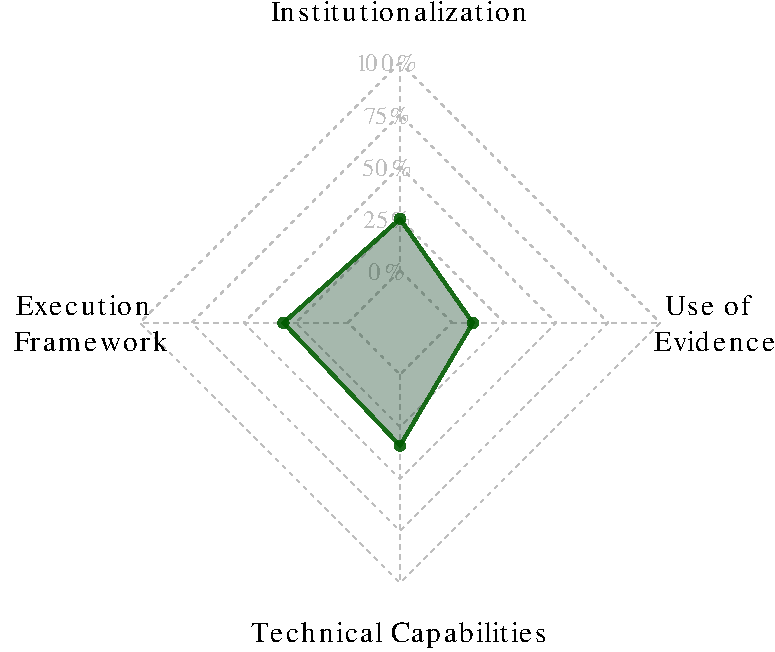
\includegraphics[width=0.7\linewidth]{_main_files/figure-latex/figure5-1} 

}

\caption{Level of progress of the Ideal RBM System}\label{fig:figure5}
\end{figure}

Considering this rate of progress, a metric was built to progressively identify five levels of maturity of RBM systems. In this way, the data presented above are averaged and a graph is generated for all the dimensions and a graph that contains the average of the dimensions, identifying the level in which the country falls . The 5 levels are:

\begin{enumerate}
\def\labelenumi{\arabic{enumi}.}
\tightlist
\item
  Early initiatives
\item
  Committed development
\item
  RBM System
\item
  Consolidated practices
\item
  Mature State
\end{enumerate}

For the case of Jamaica, the findings regarding the level of maturity of its RBM system are the following:

Jamaica is currently at the Committed development level. This occurs because even though the country has various RBM tools and activities in place, they are not articulated and regulated with a whole-of-government approach and incorporated in the planning and budgeting processes, Undoubtedly, one of the great efforts intended to correct this is the drafting of its RBM Policy, in which all government efforts will be articulated to strengthen the RBM system and obtain the expected results. However, as this Policy is not published yet, we cannot incorporate it into this diagnosis.

\hypertarget{results-by-dimension}{%
\section{Results by dimension}\label{results-by-dimension}}

The results of this diagnosis for each of the dimensions analysed (and their ideal elements) are presented below in a synthetic manner. For more detailed information on each dimension, elements, and sub-elements, please see \protect\hyperlink{appendixB}{appendix B} and visit the interactive platform with all the disaggregated findings of this PD.

\hypertarget{institutionalisation}{%
\subsection{Institutionalisation}\label{institutionalisation}}

\textbf{Key Message:}
Jamaica has regulations/frameworks to define its RBM system, identifying the relevant actors that coordinate and implement it (e.g., PMEB, PIOJ, MOFPS Performance and Monitoring Branch). However, although there are regulations/frameworks and processes in place regarding RBM, these are not articulated, so there is no connection between the RBM system and the continuous improvement of planning and budgeting decision-making to be more results-oriented.

\begingroup\fontsize{12}{14}\selectfont

\begin{tabu} to \linewidth {>{\raggedright}X>{\raggedright}X}
\hline
Ideal Element & Main results/findings\\
\hline
\textbf{1. There is a documented, approved and binding RBM Policy within the government} & Jamaica has had a long process of drafting its whole-of-government RBM Policy, and this process has incorporated inputs from different relevant stakeholders (both internal and external). In the first semester of 2022 the draft of the policy is being finalised, to be approved by the Cabinet by the end of the year.\\
\hline
\textbf{2. There are laws/regulations/norms recognizing M\&E activities across the government} & Although there are M\&E activities in some MDAs, there are no laws/regulations/norms recognizing them across all the government.\\
\hline
\textbf{3. There are guidelines that establish the rules and processes to perform monitoring activities} & The PIOJ oversees monitoring and evaluating the Medium-Term Socio-Economic Framework. For doing so, there are Technical Monitoring Committees (TMC) and thematic working groups (consultative bodies to improve planning, implementation, and monitoring). These are the only efforts to formally recognize policy monitoring in Jamaica. Though there are no guidelines regarding monitoring, there are monitoring activities across government in terms of budget and expenditure, however, in terms of the national plan and social policy, Jamaica does not have a mature set of indicators. Nevertheless, the ministries do the planning in accordance with the PMES framework.\\
\hline
\textbf{4. There are guidelines that establish the rules and processes to perform evaluation activities} & There is not a specific governing body or agency in Jamaica responsible for assisting/leading the evaluation function. However, there are some micro-projects evaluating practices within the government.\\
\hline
\textbf{5. There are guidelines that establish the rules and processes to address and use M\&E results} & Even though there are no guidelines to address and use M\&E results, budget monitoring and corporate planning are tools helping to allocate resources in priority programmes of the MDAs. However, there is no substantive use of information from M\&E to improve planning and budgeting.\\
\hline
\textbf{6. There are formal actions towards building an enabling environment} & Although there is a long way to go, Jamaica has been working on building an enabling environment for the institutionalisation, implementation, and use of an RBM system with Monitoring and Evaluation activities in its core. The GoJ has been creating incentives to use the findings of M\&E and the RBM system, such as the M\&E considerations and frameworks during the planning and budgeting processes of the MDAs (when elaborating Operational and Business Plans). However, they have not been sufficiently institutionalized to be able to obtain the expected results.\\
\hline
\textbf{7. There is a Results Oriented National Plan defined for a given period in the country} & Jamaica's National Development Plan is called Vision 2030 Jamaica and provides a comprehensive planning framework that integrates the economic, social, environmental, and governance aspects of national development. Vision 2030 is addressed in the Medium-Term Socio-Economic Policy Frameworks, which are the operationalisation of the national planning.\\
\hline
\textbf{8. There is a national budgeting strategy for a given period in the country} & There is a clear, systematic, and consistent process for the national budget.\\
\hline
\end{tabu}
\endgroup{}

\hypertarget{execution-framework}{%
\subsection{Execution Framework}\label{execution-framework}}

\textbf{Key Message:}
Jamaica has in the Office of the Cabinet the Performance Management and Evaluation Branch which acts as the coordinator of the RBM system and oversees the performance of the MDAs and harmonizing their Business Plans aligned with national objectives. The PMEB coordinates the development of a common language around M\&E and RBM, and it is recognized across government at all levels. However, to consolidate the M\&E system, it is necessary to guide and structure the processes and the management of human and financial resources to generate the evidence derived from M\&E activities that link MDAs' planning, budgeting, and implementation of their activities to achieve the desired results.

\begingroup\fontsize{12}{14}\selectfont

\begin{tabu} to \linewidth {>{\raggedright}X>{\raggedright}X}
\hline
Ideal Element & Main results/findings\\
\hline
\textbf{9. There are operative handbooks to implement the monitoring functions (i.e., Logic Framework)} & There are informal and dispersed monitoring functions in some of the MDAs, but no operative guidelines/handbooks/norms regarding Monitoring functions. However, some public agencies use monitoring tools such as the Logic Framework.\\
\hline
\textbf{10. There are operative handbooks that establish specific steps to develop each stage of the evaluation function} & There are informal and spread evaluation activities in some of the MDAs, but no operative guidelines/handbooks/norms regarding Evaluation functions.\\
\hline
\textbf{11. There is an operating and functioning coordination of M\&E at the national or/and subnational levels} & There is no formal M\&E system in Jamaica, however, the PMES works as a system for the setting of performance goals; selecting useful performance indicators and targets; reporting on results; and implementing the core components of the managing for results programme.\\
\hline
\textbf{12. There is a defined human resources structure for M\&E activities} & There are different and heterogeneous M\&E capacities among MDAs, and there are no homogeneous structures within them regarding M\&E.\\
\hline
\end{tabu}
\endgroup{}

\hypertarget{technical-capabilities}{%
\subsection{Technical capabilities}\label{technical-capabilities}}

\textbf{Key Message:}
Although there are some efforts to strengthen RBM and M\&E capabilities within the GoJ, there is no sufficient offer (both private or public) or demand (from the government) for M\&E services and capacity building in RBM. Also, there are no sufficient skilled personnel within the government with the capability to identify M\&E needs and conduct M\&E activities to orientate planning and budgeting towards results.

\begingroup\fontsize{12}{14}\selectfont

\begin{tabu} to \linewidth {>{\raggedright}X>{\raggedright}X}
\hline
Ideal Element & Main results/findings\\
\hline
\textbf{13. There are sufficient private and public entities providing M\&E services, including training, to the public sector} & Both Public and Private entities are not producing evaluations. The University of West Indies (UWI) has done some studies of public policies, probably those have some information on M\&E, but there are no verification means, as they are not publicly available. Regarding training, the Management Institute for National Development (MIND) offers a diverse set of services on performance, and hard/soft skills needed in the public sector. The Strategic and Corporate and Planning course is one of the most relevant for Jamaica in terms of some M\&E components. There has also been some training in M\&E and RBM tools, however, training is focalized in the MOFPS, Ministry of Health and Wellness, the PIOJ and the Office of the Cabinet. The PMEB has begun to implement its capacity building project with one course in MEAL recently completed. This could be extended to the rest of the government.\\
\hline
\textbf{14. There are skilled personnel in government with technical capacity and competencies to conduct planning and budgeting for results} & There are skilled personnel in government with technical capability and competencies to conduct planning and budgeting for results. However, these personnel are widely dispersed throughout the government and without the possibility (time and material resources) to effectively plan and budget for results.\\
\hline
\textbf{15. There are skilled personnel in government with technical capacity and competencies to conduct monitoring activities} & In general, there are skilled personnel in government with the technical capacity and competencies to conduct monitoring activities within the government.\\
\hline
\textbf{16. There are skilled personnel in government with technical capacity and competencies to conduct evaluations and evaluation activities} & There are few skilled personnel in government with the technical capacity and competencies to conduct evaluations and evaluation activities, and they are centralized in the MOFPS, PIOJ, and the Office of the Cabinet. These entities have personnel with the technical capacity to perform different evaluation types.\\
\hline
\end{tabu}
\endgroup{}

\hypertarget{use-of-evidence}{%
\subsection{Use of evidence}\label{use-of-evidence}}

\textbf{Key Message:}
Jamaica has some planning and budgeting information publicly available, but not regarding GoJ´s performance. Also, there are no incentives to undertake knowledge management activities and use that knowledge. The evidence derived from the RBM system and M\&E practices is not systematically included in the planning, budgeting, and implementing processes. A strategy to generate a culture of evidence use is not identified.

\begingroup\fontsize{12}{14}\selectfont

\begin{tabu} to \linewidth {>{\raggedright}X>{\raggedright}X}
\hline
Ideal Element & Main results/findings\\
\hline
\textbf{17. RBM documents and government performance information are available and accessible for consultation} & Although the RBM Policy document is not yet available, there are some documents regarding the RBM system available. However, these documents are fragmented and dispersed, so there is no alignment to have a whole of government RBM system approach.\\
\hline
\textbf{18. There is an enabling environment for the use of M\&E results} & Although there are still some challenges, there are efforts to grow and strengthen the enabling environment for the use of M\&E results within the government. Nevertheless, they are not well articulated and coordinated, so their benefits are not achieved yet.\\
\hline
\textbf{19. M\&E results are systematically included in the planning and budgeting} & M\&E results are not systematically included in the planning of Jamaica´s programmes, policies, and projects. Regarding budgeting, there is the MTRBB template and system, however, there is no information derived from M\&E contemplated when preparing the budget.\\
\hline
\textbf{20. The government has mechanisms to measure the use of the evidence that the RBM system generates} & The GoJ does not have mechanisms in place to measure the use of the evidence that the RBM system generates, both internally and externally.\\
\hline
\end{tabu}
\endgroup{}

\hypertarget{main-challenges-to-strengthen-the-rbm-system}{%
\section{Main challenges to strengthen the RBM system}\label{main-challenges-to-strengthen-the-rbm-system}}

As mentioned in \protect\hyperlink{section2}{section 2.2}, the development of an RBM System is a complex, nonlinear, and continuous process that must be contextualized in each country. In doing so, it is important to consider the main challenges that Dominica faces when it comes to strengthening its RBM system. This diagnosis identifies three major challenges:

\begin{enumerate}
\def\labelenumi{\arabic{enumi}.}
\item
  Changing the culture and fostering the enabling environment to have an RBM system in place implies a change of mindset of public servants at all levels. It should be considered that throughout the process there must be a constant awareness/sensitization strategy, both in the short and medium term, that allows public servants to identify the importance to have this mindset change in pursuit of RBM. In other words, on a regular basis, there needs to be reminders on the importance of RBM and its impact on improving performance and lives of all citizens
\item
  Since this collaboration constitutes a whole-of-government approach, it is necessary to have a top-bottom commitment in which leaders and decision-makers demonstrate the benefits of the RBM system through evidence informed actions that are generated by the RBM system. This means that we need a top-bottom approach to use, and thereby demonstrate its usefulness, the information and evidence derived from the RBM system to improve planning and budgeting decisions.
\item
  For the RBM system to be sustainable, it is critical to generate a system of incentives and ensure that there is a balance between positive and negative incentives (such as potential penalties for non-compliance), to advance and sustain the system. The positive incentives can take different forms, from monetary to symbolic, such as the presentation of awards to staff and units and recognition for good performance in public service.
\end{enumerate}

\hypertarget{section6}{%
\chapter{Next steps to building the roadmap}\label{section6}}

RBM entails more than compliance to specific requirements. Compliance is just not enough; it has to do with a change of mindset on the way things are done. This change of mindset involves different areas and stages of the administration. Having reviewed the main results from the Preparedness Diagnostic in terms of the dimensions of elements considered as part of an ideal RBM system, this section introduces the next steps that will be carried out as part of the process of building contextualized roadmaps.

The roadmap will present pathways to influence planning, budgeting, implementation, and the M\&E functions, as well as accountability and learning promotion. The main objective is for Jamaica to have a defined action course that also specifies responsibilities and shows the importance of the participation of all relevant stakeholders.

\begin{center}\rule{0.5\linewidth}{0.5pt}\end{center}

\begin{figure}

{\centering 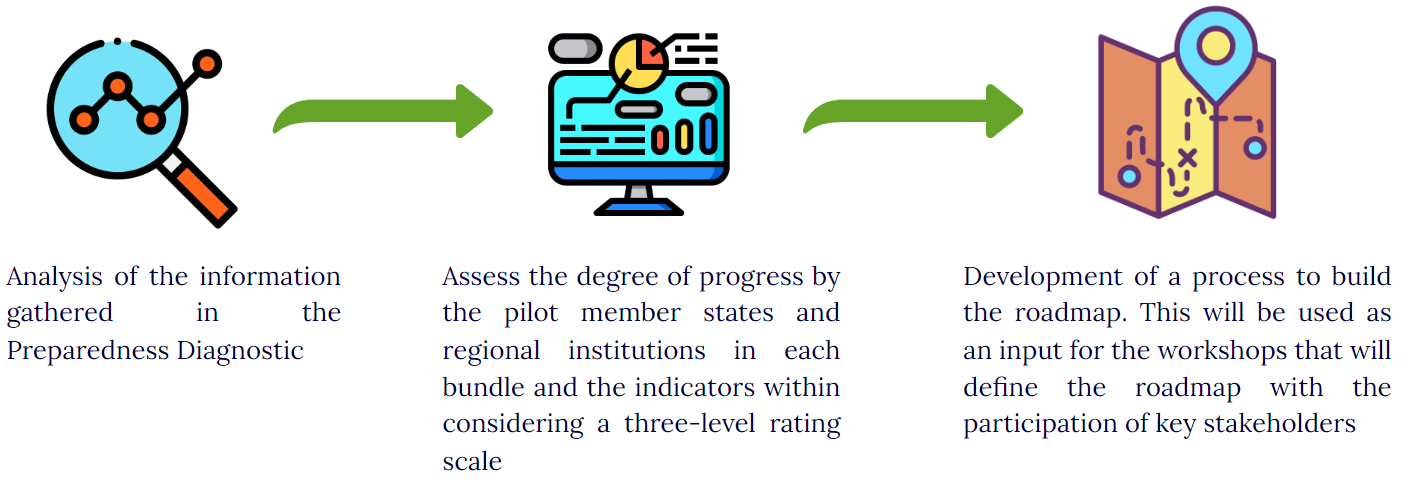
\includegraphics[width=1\linewidth]{./images/figure_6} 

}

\caption{From an ideal RBM system to the roadmaps}\label{fig:figure6}
\end{figure}

\begin{center}\rule{0.5\linewidth}{0.5pt}\end{center}

The whole process has a coproduction approach, were aside of the CLEAR LAC team, the CARICOM Secretariat, and the Executive Coordinators, key stakeholders will be involved in a fluid process to develop a learning loop for feedback and process improvement.

\begin{center}\rule{0.5\linewidth}{0.5pt}\end{center}

\begin{figure}

{\centering 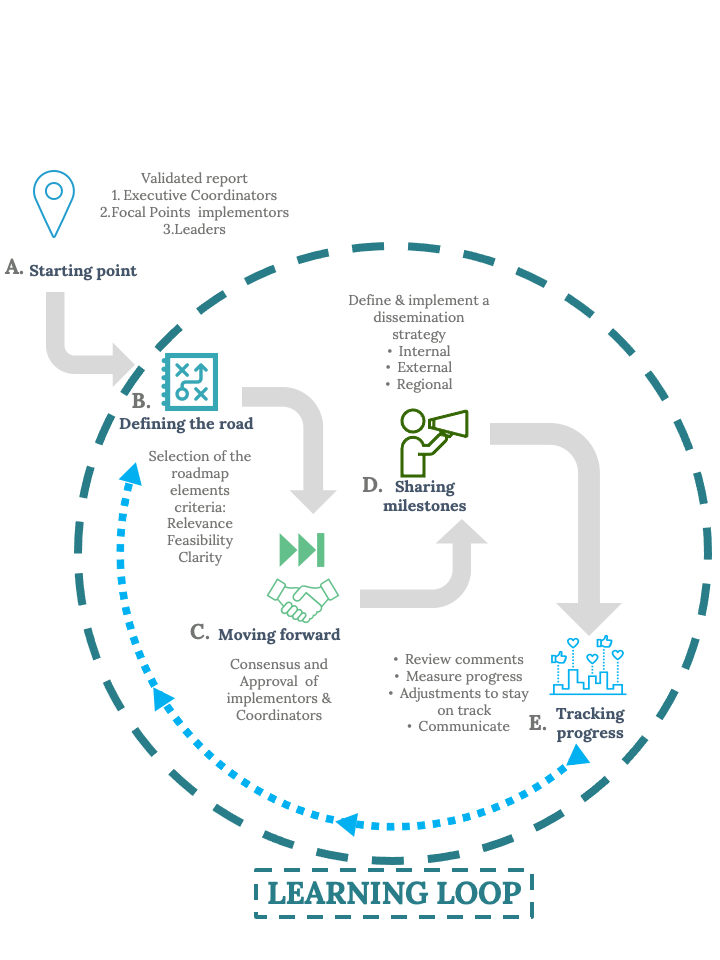
\includegraphics[width=0.75\linewidth]{./images/figure_7} 

}

\caption{Learning loop}\label{fig:figure7}
\end{figure}

\begin{center}\rule{0.5\linewidth}{0.5pt}\end{center}

This report is considered as the \emph{starting point} in this process; take into consideration that, as \protect\hyperlink{fig:figure7}{figure 7} illustrates, the process started before its publication.

Once the first draft was completed, it will be shared with key stakeholders for review and validation, starting with the Executive Coordinators. Once the feedback period concluded, the report itself became an input for what is to come and will be distributed with multiple purposes (including generating knowledge, aiding in empowering key stakeholders in the path of strengthening RBM practices, and promoting appropriation of the next steps).

The next steps start with \emph{defining the road}, engaging key stakeholders to coproduce contextualized mid-term roadmaps that will include specific activities and milestones that sought to materialize their implementation. To develop the roadmap, the CLEAR LAC team has designed a series of workshops with the participation of stakeholders involved in the different areas and levels of what is to be the national RBM system, and that have been carefully identified as part of the Preparedness Diagnostic process.

To \emph{move forward}, this first draft of the roadmap is presented to other relevant stakeholders to build a consensus and support for the process. It is crucial to gain whole-of-government ownership, so it is important to define and implement a dissemination strategy for \emph{sharing clearly define milestones} in different levels: internal, external, and regional once they have been clearly defined and responsibilities have been assigned. Finally, it is important to \emph{track the progress} of implementation and communicate results to assure that the Member State learns from the process, adjusts, and stays on the recommended path, as well as communicating results. The continuum process of identifying, sharing, reviewing, and adjusting represents a learning loop.

\hypertarget{stakeholders-contribution-analysis}{%
\section{Stakeholders' contribution analysis}\label{stakeholders-contribution-analysis}}

This section presents an analysis of stakeholders to identify which of them are relevant to strengthening the RBM system, identifying the main actors that should be involved in the process. Each of these stakeholders are involved in the decision making and execution at varied levels. Based on the CLEAR LAC's team analysis, a proposal of the possible contribution of the stakeholders (considering positions and experience) is summarised below to support the improvement of the system which will generate the necessary evidence and results for decision-making regarding planning, budgeting and thus achieve the expected results of the GoJ is presented here based on the CLEAR LAC's team analysis considering their positions and experience.

The analysis is summarized in the following table (the list of stakeholders that could take part of the RBM systems is not limited to those presented in Table 3; due to the continuous changes in dynamics within governments and other contextual factors, additional stakeholders may become relevant). During the roadmap development workshops that will be held with government stakeholders, new stakeholders could be identified or some of those presented here could be discarded. For the special case of Jamaica, it is important to recognize that, once its RBM Policy is approved and published, we will be able to have greater clarity on the roles, responsibilities, capacities, and relevance of the stakeholders that will integrate the system both at MDA and whole-of-government approach.

\begin{table}

\caption{\label{tab:unnamed-chunk-8}Stakeholders’ contribution analysis}
\centering
\fontsize{12}{14}\selectfont
\begin{tabu} to \linewidth {>{\raggedright}X>{\raggedright}X>{\raggedright}X}
\hline
Stakeholder / Position & Responsibilities / Role in the system & Incentives to be part of the system\\
\hline
\textbf{Cabinet Secretary} & •Under the direction of the Prime Minister, the Cabinet Secretary is responsible for the development, approval, and implementation of the RBM across government & •Good performance of MDAs (oversee, promote and communicate)\\
\hline
\textbf{} & •Provides direction and guidance to the Performance Monitoring and Evaluation Branch in coordinating the development and implementation of RBM frameworks and guidelines and outputs of the RBM & \\
\hline
\textbf{} & •Administers the GoJ Performance Management and Accountability System & \\
\hline
\textbf{} & •Provide leadership guidance and direction to Permanent Secretaries on the implementation of RBM & \\
\hline
\textbf{} & •Reviews the performance of Permanent Secretaries in accordance with GoJ Performance Management and Accountability guidelines & \\
\hline
\textbf{CARICOM Secretariat} & •Demand better results from the GoJ, as well as transparency and accountability & •Achieve better results to the region\\
\hline
\textbf{} & •Develop incentives for the good Member States & •Accountability to donors and governments\\
\hline
\textbf{} & •Create a best RBM practice repository and disseminate them among the Member States & \\
\hline
\textbf{} & • Generate spaces for the exchange of these best practices in the region (knowledge management) & \\
\hline
\textbf{Citizens} & •Demand better results from the government and transparency of its processes & Not Applicable\\
\hline
\textbf{Corporate Planners} & •Be the RBM Champions within their MDAs & •Fulfil what is expected from them regarding their responsibilities (planning and reporting on MDA performance)\\
\hline
\textbf{} & •Their primary function is to facilitate the efficient implementation of the Policy and results-based management practices in their respective MDAs & \\
\hline
\textbf{} & •Identify the M\&E needs of their MDAs & \\
\hline
\textbf{} & •Communicate the M\&E needs of their MDA with the RBM system coordinators & \\
\hline
\textbf{} & •Execute M\&E plans within MDAs & \\
\hline
\textbf{Management Institute for National Development} & •Be the leading institution in government training on M\&E and RBM topics, among others related to government performance & •To provide training services on M\&E and RBM and thus build better capacities in the country\\
\hline
\textbf{} & •Provide policy advice, guidance, and recommendations on the building of RBM Capacity in the Public Sector & •Gain more trust and reputation within the country\\
\hline
\textbf{} & •To fulfil their mandate to provide public servants with quality leadership development options, management training, supporting services and outreach that sustain a culture of enterprise, efficiency and responsiveness to the publics they serve. & \\
\hline
\textbf{Ministers of Government and CEOs} & •Act as a RBM Champion & •Get involved in RBM activities, such as training and sensitization will improve citizens´ perception\\
\hline
\textbf{} & •Ensure that decisions within the Ministry are based on evidence \vphantom{1} & \\
\hline
\textbf{} & •Disseminate the importance and utility of RBM in public sector \vphantom{1} & \\
\hline
\textbf{} & •Provide policy direction in its action field \vphantom{1} & \\
\hline
\textbf{Ministries, Departments and Agencies} & •The assessment and building of capacity within their organisations to operate efficiently and effectively in accordance with the RBM Policy requirements & •Comply with all the goals/results proposed in the planning of the MDA\\
\hline
\textbf{} & •Support the Change Management /transition implementation of MDAs to operating RBM Frameworks systems and approaches including: & •Get more resources for their institutions\\
\hline
\textbf{} & •Development of plans in accordance with the GoJ Integrated Planning Framework and aligned to the National Development Plan (NDP) & •Be recognized for good performance\\
\hline
\textbf{} & •Formulation of budgets in accordance with the MTRBB Framework & •Become the leaders of the sectors in which they operate\\
\hline
\textbf{} & •The building of results, monitoring and evaluation systems/frameworks in their organisations & \\
\hline
\textbf{} & •Performance Management and Accountability Systems/frameworks effectively applied in their organisations & \\
\hline
\textbf{} & •Management Information systems, performance measurement strategies, reporting, capacity, and governance structures in MDAs are consistent with the objectives of the RBM Policy/system & \\
\hline
\textbf{} & •Consider the information derived from M\&E activities in the decision-making processes & \\
\hline
\textbf{} & •Give feedback on the M\&E processes & \\
\hline
\textbf{Ministry of Finance \& Public Service} & •Provide policy direction and guidance regarding the Medium-Term Results Based Budgeting (MTRBB) Framework across the Whole of Government & •Become the leader of the results-oriented budgeting across all government\\
\hline
\textbf{} & •Regulate and monitor budgeting across government to be results oriented & •Build a strong government by strengthening the way the resources are used\\
\hline
\textbf{} & •Be the results-oriented budgeting oversee institution and advice the Prime Minister, the Cabinet and MDAs regarding budgeting & \\
\hline
\textbf{Parliament (in general)} & Review and approval of: & •Fulfil the government's counterbalancing function\\
\hline
\textbf{} & • Whole of Government Business Plan aligned to the National Budget & \\
\hline
\textbf{} & • Whole of Government Performance Report & \\
\hline
\textbf{} & • Whole of Government Evaluation Agenda & \\
\hline
\textbf{} & Review of: \vphantom{1} & \\
\hline
\textbf{} & • Strategic Business Plan of MDAs & \\
\hline
\textbf{} & • MDA Performance Reports & \\
\hline
\textbf{} & • MDA, Project Programme Evaluation Reports & \\
\hline
\textbf{} & • Demand and use M\&E information/findings to incorporate them in the parliamentary decision-making & \\
\hline
\textbf{Parliament (Public Account Committee)} & •Define needs regarding information of government performance & •Better planning of MDAs, oversee executive branch performance\\
\hline
\textbf{} & Review of: & \\
\hline
\textbf{} & •Strategic Business Plan of MDAs & \\
\hline
\textbf{} & •MDA Performance Reports & \\
\hline
\textbf{} & •MDA, Project Programme Evaluation Reports & \\
\hline
\textbf{Permanent Secretaries} & •Be responsible for ensuring that RBM and M\&E activities are effectively carried out within their MDAs & • Good performance of their respective MDAs (responsibility of the performance of MDAs)•Get involved in RBM activities, such as training and sensitization will improve citizens´ perception\\
\hline
\textbf{} & •Act as a RBM Champion and appoint the other RBM champions within MDAs & \\
\hline
\textbf{} & •Ensure that decisions within the Ministry are based on evidence & \\
\hline
\textbf{} & •Disseminate the importance and utility of RBM in public sector & \\
\hline
\textbf{} & •Provide policy direction in its action field & \\
\hline
\textbf{PIOJ chairman} & Provide policy advice and guidance to the Office of the Cabinet on the achievements regarding the goals of Vision 2030: & •Better coordination between the PIOJ (Planning governing institution) and the implementers (MDAs) of all the public interventions aiming to achieve those goals\\
\hline
\textbf{} & • GoJ Integrated Planning Framework – aligned to the National Strategic Planning Framework of the National Development Plan (NDP) and MTFs & \\
\hline
\textbf{} & • Whole-of-Government Performance Monitoring and Framework & \\
\hline
\textbf{} & • Whole of Government Performance Management Information Strategy & \\
\hline
\textbf{} & • In collaboration with the Office of the Cabinet, the Ministry of Finance and the Public Service and the Auditor Generals Department undertakes the evaluations of Whole of Government Performance & \\
\hline
\textbf{} & • Ensures that National Development Programmes administered by the PIOJ are implemented in accordance with the requirements of the RBM Policy & \\
\hline
\textbf{} & •Better coordination between the PIOJ (Planning governing institution) and the implementers (MDAs) of all the public interventions aiming to achieve those goals & \\
\hline
\textbf{} & • With the PMEB, define the universe of evaluation (what to evaluate, how, when and who) & \\
\hline
\textbf{Performance Management and Evaluation Branch CTD} & •Generate frameworks, guidelines and coordinate RBM activities across government and other relevant stakeholders, such as the MIND, PIOJ, MOFPS, etc. & •Achieve the complete rollout of the RBM practices within government\\
\hline
\textbf{} & • Coordinate with the MOFPS and the PIOJ so as not to overlap monitoring objects and monitoring periods & •Become the leader of the results-oriented planning across all government and then strengthen the government in the areas of planning, budgeting and implementing for results (with specific responsibility on planning)\\
\hline
\textbf{} & •Define mechanisms to comprehensively monitor and evaluate programmes & \\
\hline
\textbf{} & •Follow up on the roadmap worked on for the implementation of the RBM system and report progress to different audiences: leaders, MDAs and citizens & \\
\hline
\textbf{} & • With the PIOJ, define the universe of evaluation (what to evaluate, how, when and who) & \\
\hline
\textbf{Prime Minister} & •As the Chief Executive is the Sponsor/Champion for the development and implementation of the RBM Policy & • Whole of Government performance improved\\
\hline
\textbf{} & •Provide policy direction with respect to the development of the results Based Management across the Public Sector & • Improve the perception that citizens have regarding the performance of the government\\
\hline
\textbf{} & • Instruct the actions of the RBM and appoint system coordinators & •Improve confidence/trust with the external sector: investors, donors, etc.\\
\hline
\textbf{} & •Disseminate the RBM strategy to the public & \\
\hline
\textbf{Universities} & •Use the results of the M\&E processes & •Offer RBM/M\&E training to public servants (increase earnings)\\
\hline
\textbf{}\textbf{} & •Participate in the M\&E processes of the government & •Offer RBM/M\&E services to government (increase earnings and strengthening the community of practice in the country and the region)\\
\hline
\textbf{} & •Offer M\&E services both in training and monitoring and evaluating & \\
\hline
\textbf{} & •Demand evidence derived from M\&E \vphantom{1} & \\
\hline
\textbf{} & •Keep the GoJ accountable \vphantom{1} & \\
\hline
\textbf{VOPE (Caribbean Evaluators International)} & •Use the results of the M\&E processes & •Offer RBM/M\&E training to public servants\\
\hline
 & •Participate in the M\&E processes of the government & •Offer RBM/M\&E services to government\\
\hline
\textbf{} & •Offer M\&E services both in training and monitoring and evaluating & •Strengthening the community of practice in the country and the region)\\
\hline
\textbf{} & •Demand evidence derived from M\&E & \\
\hline
\textbf{} & •Keep the GoJ accountable & \\
\hline
\multicolumn{3}{l}{\rule{0pt}{1em}\textit{Note: }}\\
\multicolumn{3}{l}{\rule{0pt}{1em}Developed by the CLEAR LAC technical team in charge of the collaboration}\\
\end{tabu}
\end{table}

\hypertarget{references-sources}{%
\chapter*{References \& Sources}\label{references-sources}}
\addcontentsline{toc}{chapter}{References \& Sources}

\begin{itemize}
\item
  Bank of Jamaica. Monthly inflation highlights. Consulted in: \url{https://boj.org.jm/core-functions/monetary-policy/what-is-inflation/} .
\item
  BBC News. (January 10, 2018). Jamaica country profile. \url{https://www.bbc.com/news/world-latin-america-18784061}
\item
  Black, C. V., Ferguson, J. A., \& Bryan, P. (n.~d.). Jamaica - Government and society. Encyclopaedia Britannica. Consulted in: \url{https://www.britannica.com/place/Jamaica/Government-and-society}
\item
  Centro de Estudios Internacionales Gilberto Bosques. (April, 2020). Jamaica Ficha Técnica. Consulted in: \url{https://centrogilbertobosques.senado.gob.mx/docs/F_Jamaica.pdf}
\item
  Food and Agriculture Organization of the United Nations. \url{https://www.fao.org/investment-learning-platform/themes-and-tasks/results-based-management/en/\#c309481}
\item
  Jamaica General Election Results 2016. (February 17, 2022). Knowledge Walk Institute. Consulted in: \url{http://www.caribbeanelections.com/jm/elections/jm_results_2016.asp}
\item
  Ministerio de Asuntos Exteriores de España. (October, 2021). Ficha País Jamaica. Consulted in: \url{http://www.exteriores.gob.es/Documents/FichasPais/Jamaica_FICHA\%20PAIS.pdf}
\item
  United Nations Development Group. Results-Based Management Handbook. \url{https://unsdg.un.org/download/160/246\#}:\textasciitilde:text=RBM\%20is\%20a\%20management\%20strategy,higher\%20level\%20goals\%20or\%20impact).
\item
  United Nations Development Programme. Results Based Management. Concepts and Methodology. \url{http://web.undp.org/evaluation/documents/RBMConceptsMethodgyjuly2002.pdf}
\item
  Overview. (April 13, 2020). World Bank.
  World Bank. Country Overview, Jamaica. Consulted in: \url{https://www.worldbank.org/en/country/jamaica/overview\#1}
\item
  World Bank. Return to paradise: A poverty perspective on Jamaica's COVID-19 recovery response. Consulted in: \url{https://blogs.worldbank.org/latinamerica/return-paradise-poverty-perspective-jamaicas-covid-19-recovery-response} , with data from the Statistical Institute of Jamaica.
\end{itemize}

The rest of the sources are official websites of the Government of Jamaica or regional institutions/initiatives, such as (but not limited only):

\begin{itemize}
\item
  Caribbean Development Portal. \url{http://www.jamstats.gov.jm/}
\item
  Government of Jamaica. \url{https://www.gov.jm/}
\item
  House of Parliament. \url{https://www.japarliament.gov.jm/}
\item
  JamStats Secretariat. \url{http://www.jamstats.gov.jm/}
\item
  Ministry Of Agriculture and Fisheries. \url{https://www.moa.gov.jm/}
\item
  Ministry Of Culture, Gender, Entertainment and Sport. \url{https://mcges.gov.jm/}
\item
  Ministry Of Economic Growth and Job Creation. \url{https://megjc.gov.jm/}
\item
  Ministry Of Education and Youth. \url{https://moey.gov.jm/}
\item
  Ministry of Finance and the Public Service. \url{https://mof.gov.jm/}
\item
  Ministry Of Foreign Affairs and Foreign Trade. \url{https://mfaft.gov.jm/jm/}
\item
  Ministry Of Health and Wellness. \url{https://www.moh.gov.jm/}
\item
  Ministry Of Industry, Investment and Commerce. \url{https://www.miic.gov.jm/}
\item
  Ministry Of Justice. \url{https://moj.gov.jm/}
\item
  Ministry of Labour and Social Security. \url{https://mlss.gov.jm/}
\item
  Ministry Of Legal and Constitutional Affairs. \url{https://jis.gov.jm/government/ministries/legal-and-constitutional-affairs/}
\item
  Ministry Of Local Government and Rural Development. \url{https://www.localgovjamaica.gov.jm/}
\item
  Ministry Of National Security. \url{https://www.mns.gov.jm/}
\item
  Ministry Of Science, Energy and Technology. \url{https://www.mset.gov.jm/}
\item
  Ministry Of Tourism. \url{https://www.mot.gov.jm/}
\item
  Ministry Of Transport and Mining. \url{https://mtm.gov.jm/}
\item
  Office of the Cabinet. \url{https://cabinet.gov.jm/}
\item
  Office Of the Prime Minister. \url{https://opm.gov.jm/}
\item
  The Management Institute for National Development. \url{https://mind.edu.jm/}
\end{itemize}

\hypertarget{appendix-appendix}{%
\appendix}


\hypertarget{appendixA}{%
\chapter{Conceptual framework (CLEAR LAC)}\label{appendixA}}

\hypertarget{key-dimensions-of-a-sustainable-rbm-system}{%
\section{Key dimensions of a sustainable RBM System}\label{key-dimensions-of-a-sustainable-rbm-system}}

The development of an RBM System is a complex and nonlinear process that must be contextualized to the specific region, country, or regional institution. However, the multiple efforts done over time allow us to learn from experiences in different settings and identify good practices. These good practices represent useful inputs to be considered when embarked on this road.

One significant component to strengthen RBM in the Community is to build, in a participatory process, specific roadmaps to continue the development of RBM Systems for each pilot member state and regional institution. The member states and regional institutions participating in the pilot have significant but heterogeneous advances achieving this goal. To identify these advances and guide the analysis of the Preparedness Diagnostic stages, the CLEAR LAC team defined four dimensions of an ideal and sustainable RBM System:

\begin{itemize}
\item
  \emph{Institutionalisation:} this dimension focuses on the formal rules that defines, outlines and formalize the RBM Systems in the countries.
\item
  \emph{Execution framework:} this dimension focuses on the systems, resources, processes, methodologies, and tools necessary for the implementation of the RBM system, as well as incentives that promote an enabling environment.
\item
  \emph{Technical capabilities:} this dimension focuses on the capacities, abilities, and resources necessary to implement and sustain the RBM System.
\item
  \emph{Use of evidence:} this dimension focuses on the dissemination strategies and incentives aimed at stakeholders with the purpose that they use the evidence generated by the RBM System and its measurement.
\end{itemize}

\hypertarget{ideal-elements-sub-elements}{%
\section{Ideal elements \& sub-elements}\label{ideal-elements-sub-elements}}

The four dimensions previously mentioned were conceptualized as necessary components when building an operating and sustainable RBM system. To have a better understanding of what the progress in each dimension entails, we propose a set of ideal elements and sub-elements taken from different contexts and experiences where they have been successfully implemented or recommended. Each dimension has a set of elements that represent activities, documents, normative frameworks, skills, incentives, etc.; and every element has a set of sub-elements that describe the ideal characteristics of the element. The sub-elements allow to translate concepts into practice, and, after gathering and analysing information, this knowledge can be translated into specific actions.

Unlike the dimensions, as RBM Systems are designed and built considering contextual factors, some elements and sub-elements should be taken as a guide as different contexts will result in variations on their interpretation and level of relevance/priorities. This framework allows for adaptations, recognizing that every context is particular and that there is no unique checklist that may apply to all contexts.

\begin{table}
\centering
\begin{tabular}[t]{l}
\hline
I. Institutionalisation Ideal elements\\
\hline
\multicolumn{1}{l}{\textbf{1. There is a documented, approved and binding RBM Policy within the government:}}\\
\hline
\hspace{1em}It is relevant across the government at all levels\\
\hline
\hspace{1em}It outlines guiding principles / pillars that are alligned to a results-oriented approach\\
\hline
\hspace{1em}It communicates what RBM entails (i.e., clear definitions for key concepts) and clearly states how it works\\
\hline
\hspace{1em}It identifies key actors who are responsible for the coordination and the measurement of the overall results of the RBM policy\\
\hline
\hspace{1em}It identifies key actors who are responsible for supervising the implementation of the RBM policy and their functions (within the MDAs)\\
\hline
\hspace{1em}It is use-oriented in planning, budgeting and implementing towards results (cronograma)\\
\hline
\hspace{1em}The funding for M\&E activities and the responsibles are identified\\
\hline
\multicolumn{1}{l}{\textbf{2. There are laws/regulations/norms* recognizing M\&E activities across the government}}\\
\hline
\hspace{1em}They are aditional to the RBM Policy\\
\hline
\hspace{1em}They delegate M\&E responsibilities to a single national body or to multiple MDAs\\
\hline
\hspace{1em}It is relevant across the government at all levels and branches (i.e. scope of action) and defines the M\&E subjects\\
\hline
\hspace{1em}They stablish that the M\&E results affect planning, budgeting and implementing activities\\
\hline
\hspace{1em}(If more than one) They are consistent with each other\\
\hline
\hspace{1em}It stablishes the need to designate focal points in each MDA across government\\
\hline
\multicolumn{1}{l}{\textbf{3. There are guidelines that establish the rules and processes to perform monitoring activities:}}\\
\hline
\hspace{1em}•They identify indicator types and the dimensions they want to measure (e.g., efficiency, efficacy), and monitoring tools (e.g., logic framework) to be developed for each project / social programme\\
\hline
\hspace{1em}•They identify specific timeframes to collect indicator data and develop monitoring tools to measure the indicators (e.g., collect every six months) for each project\\
\hline
\hspace{1em}They have criteria to ensure data collection quality (design, measurement, report)\\
\hline
\hspace{1em}They integrate the indicators as a monitoring system\\
\hline
\hspace{1em}The monitoring system has a stablished process to update its information periodically\\
\hline
\hspace{1em}The monitoring system has a stablished process to update its indicators periodically\\
\hline
\hspace{1em}There are rules providing all parts in the monitoring process with a way of presenting their opinion (i.e. institutional positions)\\
\hline
\multicolumn{1}{l}{\textbf{4. There are guidelines that establish the rules and processes to perform evaluation activities:}}\\
\hline
\hspace{1em}They identify key stakeholders  to be part of the evaluation process (e.g. evaluation process coordinators, evaluation subjects, evaluation process implementators)\\
\hline
\hspace{1em}They identify specific evaluation types\\
\hline
\hspace{1em}The identify specific timeframes for each evaluation type\\
\hline
\hspace{1em}They identify specific characteristics and functions of evaluators\\
\hline
\hspace{1em}It establishes an iterative process of evaluation (i.e. is not a one-time exercise)\\
\hline
\hspace{1em}They identify the elements to be included in the evaluation's ToRs (e.g. objectives of the evaluation, the role and responsibilities of the evaluator and evaluation client and the resources available to conduct the evaluation)\\
\hline
\hspace{1em}They outline the operationalization process of the national evaluation agenda (i.e. it is agreed among relevant stakeholders)\\
\hline
\hspace{1em}There have quality control mechanisms for evaluation activities (e.g. quality attribute listings, quality evaluations, peer review, satisfaction surveys, evaluate the evaluator)\\
\hline
\hspace{1em}There are rules providing all parts in the evaluation process with a way of presenting their opinion (i.e. institutional position)\\
\hline
\multicolumn{1}{l}{\textbf{5. There are guidelines that establish the rules and processes to address and use of M\&E results}}\\
\hline
\hspace{1em}They identify instruments to measure the RBM System results\\
\hline
\hspace{1em}They identify mechanisms to use monitoring results\\
\hline
\hspace{1em}They identify mechanisms to use evaluation results\\
\hline
\hspace{1em}They establish rules and processes that require the budgeting process to consider the results of M\&E activities (they make explicit the link between planning and budgeting)\\
\hline
\multicolumn{1}{l}{\textbf{6. There are formal actions towards building an enabling environment}}\\
\hline
\hspace{1em}There are key stakeholders identified as responsibles for these formal actions.\\
\hline
\hspace{1em}There are strategies to enhance or attenuate possitive or negative incentives for the use of monitoring\\
\hline
\hspace{1em}There are strategies to enhance or attenuate possitive or negative incentives for the use of evaluation\\
\hline
\hspace{1em}There are mechanisms for the participation of stakeholders in the definition of monitoring activities and needs\\
\hline
\hspace{1em}There are mechanisms for the participation of stakeholders in the definition of evaluation activities and needs\\
\hline
There are periodic meetings involving relevant stakeholders to review the M\&E
\hspace{1em}information as an RBM System feedback exercise\\
\hline
\hspace{1em}There is a permanent strategy to communicate and sensitize about the benefits and challenges of RBM.\\
\hline
\multicolumn{1}{l}{\textbf{7. There is a Results Oriented National Plan defined for a given period in the country:}}\\
\hline
\hspace{1em}It has defined objectives\\
\hline
\hspace{1em}It is constructed in a participatory process\\
\hline
\hspace{1em}It is constructed using the information generated by the RBM System\\
\hline
\hspace{1em}  It has defined strategies to implement the plan\\
\hline
\hspace{1em}  It has defined indicators and monitoring tools by mandate, and they measure outcomes and outputs\\
\hline
\hspace{1em}It is evaluated by mandate\\
\hline
\hspace{1em}It  has specific evaluation activities\\
\hline
\hspace{1em}  It has defined responsible actors\\
\hline
\hspace{1em}  It considers regional (CARICOM) objectives\\
\hline
\multicolumn{1}{l}{\textbf{8. There is a national budgeting strategy for a given period in the country:}}\\
\hline
\hspace{1em}It is allocated according to the objectives/goals/activities of the national planning\\
\hline
\hspace{1em}It considers the prioritization of the objectives/goals/activities identified in the national planning\\
\hline
\hspace{1em}It is allocated and updated using the information generated by evidence and the RBM System\\
\hline
\hspace{1em}The budget allocation is defined in annual terms (i.e. it specify the starting date, relevant milestones dates, and the end date)\\
\hline
\hspace{1em}It stabishes a specific allocation of resources for M\&E activities according to the budget period\\
\hline
\hspace{1em}It considers other available information to define its allocation (e.g national statistics/poverty measurements/etc, CARICOM)\\
\hline
\hspace{1em}The key actors and their responsibilities are clearly defined\\
\hline
\end{tabular}
\end{table}

\begin{table}
\centering
\begin{tabular}[t]{l}
\hline
II. Excecution Framework Ideal elements\\
\hline
\multicolumn{1}{l}{\textbf{9. There are operative handbooks to implement the monitoring functions (i.e. Logic Framework):}}\\
\hline
\hspace{1em}They identify all the relevant activities to develop each stage of the process (e.g.specific activities within the analysis of the project's context, stakeholder)\\
\hline
\hspace{1em}They outline specific timeframes to implement every stage of the \vphantom{1} process\\
\hline
\hspace{1em}They identify the responsibles in every stage of the process (specific MDAs and units within the MDAs)\\
\hline
\hspace{1em}They outline a dissemination strategy of the LF results (what, how, when and to who do you want to diffuse the results)\\
\hline
\hspace{1em}The indicators are oriented to results and outcomes\\
\hline
\multicolumn{1}{l}{\textbf{10. There are operative handbooks that establish specific steps to develop each stage of the evaluation function:}}\\
\hline
\hspace{1em}They identify all the relevant activities to develop each stage of the evaluation process (e.g. evaluators selection, ToR definition for each evaluation, evaluation supervision)\\
\hline
\hspace{1em}They outline specific timeframes to implement every stage of the process\\
\hline
\hspace{1em}They outline a dissemination strategy of the evaluation results (what, how, when and to who do you want to diffuse the results)\\
\hline
\hspace{1em}They identify the responsible (specific MDAs and units within the MDAs)  in every stage of the process\\
\hline
\multicolumn{1}{l}{\textbf{11. There is an operating and functioning coordination of M\&E at the national or/and subnational levels:}}\\
\hline
\hspace{1em}It is homogeneous across the government and holds a common language in concepts of M\&E\\
\hline
\hspace{1em}It is integrated at various levels of government (national and subnational)\\
\hline
\hspace{1em} It is known by all sectors and MDAs* in government\\
\hline
\hspace{1em}It is relevant (e.g. it recollects indicator data that is necessary, pertinent, and timely, it involves key stakeholders at different levels)*\\
\hline
\hspace{1em}It generates timely documents for specific evidence users*\\
\hline
\hspace{1em}It generates use-oriented documents for specific evidence users*\\
\hline
\hspace{1em}It is sufficiently funded (specific financial resources are allocated)\\
\hline
\multicolumn{1}{l}{\textbf{12. There is a defined human resources structure for M\&E activities:}}\\
\hline
\hspace{1em}It has specific focal points in each MDA across the government\\
\hline
\hspace{1em}The MDA focal points constitute a coordinated network that is part of the M\&E System\\
\hline
\hspace{1em}The MDA focal points have clear functions, responsibilities and expected outcomes\\
\hline
\hspace{1em}The MDAs focal points become  recognized strategic areas of information about the performance and impact of the MDAs projects / programmes.\\
\hline
\end{tabular}
\end{table}

\begin{table}
\centering
\begin{tabular}[t]{l}
\hline
III. Technical Capabilities Ideal elements\\
\hline
\multicolumn{1}{l}{\textbf{13. There are sufficient private and public entities providing M\&E services, including training, to the public sector.}}\\
\hline
\hspace{1em}They provide a variety of M\&E services (e.g conduct diagnostics, evaluations, assessments)\\
\hline
\hspace{1em}MDAs demand those M\&E services based on their needs\\
\hline
\hspace{1em}They provide a broad academic offer for RBM capacity building (e.g continous courses / diplomas in M\&E topics, specific training to the public sector )\\
\hline
\hspace{1em}There is an M\&E capacity building strategy demanding RBM training, that is periodic, targeted to the capacity building needs and with a whole-of-government approach\\
\hline
\multicolumn{1}{l}{\textbf{14. There are skilled personnel in government with technical capacity and competencies to conduct planning and budgeting for results:}}\\
\hline
\hspace{1em}They have technical skills to use derived evidence from M\&E to improve planning (identify priorities, vulnerable population, what works to attend that priorities)\\
\hline
\hspace{1em}They have competences to use M\&E results to define results-oriented budgeting ( e.g., identify priorities, new public problems that should be adressed, policies that work, compare between policies), as well as soft\\
\hline
\hspace{1em}They have competences to coordinate with other MDAs and relevant actors\\
\hline
\multicolumn{1}{l}{\textbf{15. There are skilled personnel in government with technical capacity and competencies to conduct monitoring activities:}}\\
\hline
\hspace{1em}They have technical skills to collect indicator data\\
\hline
\hspace{1em}They have technical skills to use monitoring tools\\
\hline
\hspace{1em}They have the competences to identify monitoring needs in order to collect relevant, pertinent and timely data\\
\hline
\multicolumn{1}{l}{\textbf{16. There are skilled personnel in government with technical capacity and competencies to conduct evaluations and evaluation activities:}}\\
\hline
\hspace{1em}They have the competences to perform different evaluation types (e.g. design, process, impact) and use different methodologies (i.e., quantitative, qualitative, mixed-methods)\\
\hline
\hspace{1em}They have the competences to identify evaluation needs and match them with proper evaluation types and methodologies: define evaluation horizon and ask relevant evaluation questions\\
\hline
\hspace{1em}They have the competences to formulate reports that include relevant, pertinent and timely information for different stakeholders\\
\hline
\hspace{1em}There is a capacity strengthening plan for on-going training in RBM and M\&E\\
\hline
\end{tabular}
\end{table}

\begin{table}
\centering
\begin{tabular}[t]{l}
\hline
IV. Use of Evidence Ideal elements\\
\hline
\multicolumn{1}{l}{\textbf{17. RBM documents and goverment performance information are available and accesible for consultation}}\\
\hline
\hspace{1em}National planning documents are publicly available\\
\hline
\hspace{1em}National budget plans are publicly available\\
\hline
\hspace{1em}Documents that mention the results/findings/recommendations of monitoring and evaluation activities are publicly available\\
\hline
\hspace{1em}M\&E manuals / guidelines /ToRs are publicly available\\
\hline
\hspace{1em}There is a dissemination strategy of evidence about government performance targeted to different stakeholders (e.g. citizens, parlamentarians, decision makers, private sector, NGOs)\\
\hline
\multicolumn{1}{l}{\textbf{18. There is an enabling environment for the use of M\&E results:}}\\
\hline
\hspace{1em}There are explicit possitive or negative incentives for the use of monitoring results\\
\hline
\hspace{1em}There are explicit possitive or negative incentives for the use of evaluation results\\
\hline
\hspace{1em}There are knowledge management practices\\
\hline
\multicolumn{1}{l}{\textbf{19. M\&E results are systematically included in the planning \& budgeting:}}\\
\hline
\hspace{1em}They are used in an institutionalized way: they follow a established procedure\\
\hline
\hspace{1em}There are action plans or other management instruments to ensure M\&E results/recommendations are implemented\\
\hline
\hspace{1em}They justify the creation and design of government interventions\\
\hline
\hspace{1em}They identify the target population of government interventions\\
\hline
\hspace{1em}They identify general and specific recommendations to improve the implementation of government interventions\\
\hline
\hspace{1em}They inform the design/redesign of government interventions\\
\hline
\hspace{1em}They inform the initial budget allocations of government interventions\\
\hline
\hspace{1em}They inform the budget increase/decrease/suspension of government interventions\\
\hline
\hspace{1em}Evaluation findings/reports are updated periodically\\
\hline
\hspace{1em}The M\&E results are used to define the MDAs budget\\
\hline
\multicolumn{1}{l}{\textbf{20. The governemt has mechanisms to measure the use of the evidence that the RBM system generates}}\\
\hline
\hspace{1em}There are mechanisms to know how much the reports and publications on M\&E are downloaded or used by citizens\\
\hline
\hspace{1em}There are use-of-evidence measurements to improve the use of M\&E results strategy\\
\hline
\end{tabular}
\end{table}

\hypertarget{levels-of-progress}{%
\section{Levels of progress}\label{levels-of-progress}}

The Preparedness Diagnostic methodology is designed to gain a deep understanding of a country or institution's relevant aspects/characteristics when developing an RBM System. The different stages are meant to gather information from different stakeholders to achieve a whole of government / institutional outlook. The dimensions with ideal elements and sub-elements guide the analysis of the information gathered in order to identify the level of progress of a specific government or institution.

The scale used to assess the sub-elements are:

\begin{itemize}
\tightlist
\item
  No: there is no documented advance in the sub-element
\item
  Needs improvement: there is documented advance in the sub-element, but do not cover all the criteria express in the sub-element.
\item
  Yes: there is documented proof that the sub-element complies with the needed/ideal characteristics
\end{itemize}

Each scale level has an assigned value, and every element will have a result obtained from the total sum of its sub-element's scores. The average score of the elements per dimension results in the dimension's score, and the average score of the four dimensions will place the Member state/regional Institution in one of the following \textbf{levels of progress} of their RBM Systems:

\begin{itemize}
\tightlist
\item
  Level 0. No RBM
\item
  Level 1. Early initiatives: there are some initiatives to develop RBM-related structures and focus on monitoring activities
\item
  Level 2. Committed development: there are RBM-related structures being stablished and limited evaluation activities
\item
  Level 3.. Growing RBM system: there are RBM-related structures being stablished and limited evaluation activities
\item
  Level 4. Consolidated practices: there are integrated efforts (political will, capacity building and some whole-of-government consensus) to develop the RBM System
\item
  Level 5. Mature state: Functioning and sustainable RBM System in place that generates credible, reliable and timely information that improves public policies
\end{itemize}

\begin{center}\rule{0.5\linewidth}{0.5pt}\end{center}

\begin{figure}

{\centering 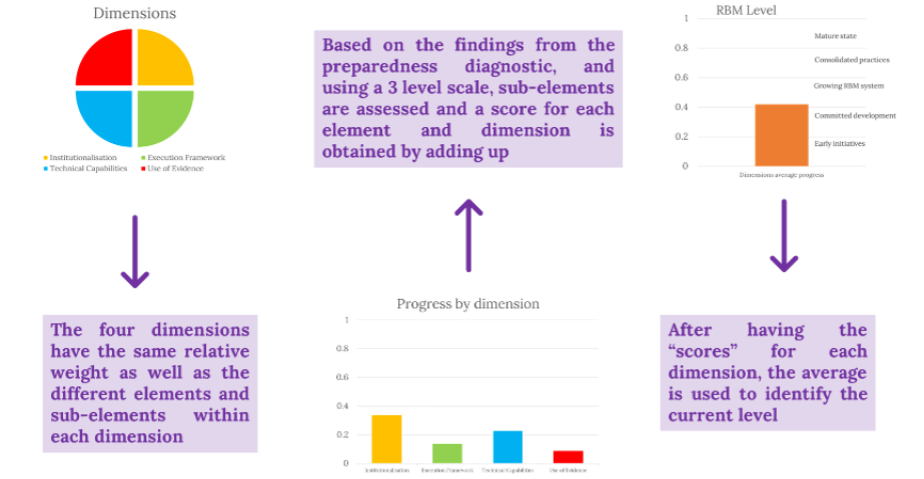
\includegraphics[width=1\linewidth]{./images/figure_8} 

}

\caption{How to identify the current level of the RBM system maturity}\label{fig:figure8}
\end{figure}

\begin{center}\rule{0.5\linewidth}{0.5pt}\end{center}

\hypertarget{appendixB}{%
\chapter{Detailed findings}\label{appendixB}}

In the following table, you can consult all the findings found in this PD in detail.

\begin{table}
\centering
\begin{tabular}[t]{l|l}
\hline
I. Institutionalisation Detailed Findings &  \\
\hline
\multicolumn{2}{l}{\textbf{1. There is a documented, approved and binding RBM Policy within the government:}}\\
\hline
\hspace{1em}1.1 It is relevant across the government at all levels & Throughout the PD process it was mentioned that the RBM Policy will be relevant across the government at all levels.\\
\hline
\hspace{1em}1.2 It outlines guiding principles / pillars that are aligned to a results-oriented approach & Throughout the PD process it was mentioned that the RBM Policy will present guiding principles that are aligned to a results-oriented whole-of-government approach.\\
\hline
\hspace{1em}1.3 It communicates what RBM entails (e.g., clear definitions for key concepts) and clearly states how it works & Throughout the PD process it was mentioned that the RBM Policy will communicate what TBM entails and will contain definitions of the main concepts and ideas regarding RBM, M\&E and Performance.\\
\hline
\hspace{1em}1.4 It identifies key actors who are responsible for the coordination and the measurement of the overall supervision and coordination of the RBM policy & Throughout the PD process it was mentioned that the RBM Policy will present a matrix of RBM key stakeholders, identifying their explicit role as a part of the RBM system.\\
\hline
\hspace{1em}1.5 It identifies key actors who are responsible for supervising the implementation of the RBM policy and their functions (within MDAs) & Throughout the PD process it was mentioned that the RBM Policy will present a matrix of RBM key stakeholders, identifying their explicit role as a part of the RBM system and within their respective MDAs.\\
\hline
\hspace{1em}1.6 It is use-oriented in planning, budgeting, and implementing towards results, transparency and accountability & Allegedly, the RBM Policy will articulate RBM/M\&E practices with the processes of planning, budgeting, and therefore transparency and accountability.\\
\hline
\hspace{1em}1.7 The funding for M\&E activities and the responsible are identified & Allegedly, the RBM Policy will state how the system will be funded.\\
\hline
\multicolumn{2}{l}{\textbf{2. There are laws/regulations/norms* recognizing M\&E activities across the government}}\\
\hline
\hspace{1em}2.1 They are additional to the RBM Policy & Not Applicable\\
\hline
\hspace{1em}2.2 They delegate M\&E responsibilities to a single national body or to multiple MDAs & Although there are no laws/regulations/norms recognizing M\&E activities across the government, the MOFPS has the Performance and Monitoring Branch, which is responsible for the monitoring, on a monthly basis, of the budgeting reports of agencies and departments.\\
\hline
\hspace{1em}2.3 It is relevant across the government at all levels and branches (e.g., scope of action) and defines the M\&E subjects & Not Applicable\\
\hline
\hspace{1em}2.4 They stablish that the M\&E results affect planning, budgeting and implementing activities & Not Applicable\\
\hline
\hspace{1em}2.5 (If more than one) They are consistent with each other & Not Applicable\\
\hline
\hspace{1em}2.6 It stablishes the need to designate focal points in each MDA across government & Not Applicable\\
\hline
\multicolumn{2}{l}{\textbf{3. There are guidelines that establish the rules and processes to perform monitoring activities:}}\\
\hline
\hspace{1em}3.1 They identify indicator types and the dimensions they want to measure (e.g. efficiency, efficacy), and monitoring tools (e.g. logic framework) to be developed for each project / social programme & The National Plan (Jamaica Vision 2030) has a set of defined indicators for some sectors, and its updating depends on data availability. Jamaica has data for development initiatives to be able to have a full set of indicators and to make them accessible.\\
\hline
\hspace{1em}3.2 They identify specific timeframes to collect indicator data and develop monitoring tools to measure the indicators (e.g., collect every six months) for each project & Vision 2030 does have a set of indicators, timeframes and the responsible MDAs to ensure data collection but there are no instruments in place to systematize M\&E results/findings/data.\\
\hline
\hspace{1em}3.3 They have criteria to ensure data collection quality (design, measurement, report) & There are no systems to generate, understand and use data. Jamaica has strategic planning templates that are used by all Ministries. Departments and Agencies are guided by the Minimum Standards. This use is based on compliance basis and the information is not always used to improve planning and budgeting.\\
\hline
\hspace{1em}3.4 They integrate the indicators as a monitoring system & Vision 2030 does have a set of indicators, timeframes and the responsible MDAs to ensure data collection but there are no instruments in place to systematize M\&E results/findings/data.\\
\hline
\hspace{1em}3.5 The monitoring system has a stablished process to update its information periodically & There are budget information reports generated periodically, but there is no evidence that MDAs update KPIs information periodically.\\
\hline
\hspace{1em}3.6 The monitoring system has a stablished process to update its indicators periodically & NA\\
\hline
\hspace{1em}3.7 There are rules providing all parts in the monitoring process with a way of presenting their opinion (e.g., institutional positions) & NA\\
\hline
\multicolumn{2}{l}{\textbf{4. There are guidelines that establish the rules and processes to perform evaluation activities:}}\\
\hline
\hspace{1em}4.1 They identify key stakeholders to be part of the evaluation process (e.g., evaluation process coordinators, evaluation subjects, evaluation process implementors) & When evaluating the Medium-Term Socio-Economic Framework, the PIOJ considers which MDAs are responsible for implementing programmes, and then identify the responsible who should answer for the information requested regarding programmes´ goals.\\
\hline
\hspace{1em}4.2 They identify specific evaluation types & NA\\
\hline
\hspace{1em}4.3 The identify specific timeframes for each evaluation type & NA\\
\hline
\hspace{1em}4.4 They identify specific characteristics and functions of evaluators & NA\\
\hline
\hspace{1em}4.5 It establishes an iterative process of evaluation (e.g.,  is not a one-time exercise) & NA\\
\hline
\hspace{1em}4.6 They identify the elements to be included in the evaluation's ToRs (e.g., objectives of the evaluation, the role and responsibilities of the evaluator and evaluation client and the resources available to conduct the evaluation) & NA\\
\hline
\hspace{1em}4.7 They outline the operationalization process of the national evaluation agenda (e.g., it is agreed among relevant stakeholders) & NA\\
\hline
\hspace{1em}4.8 There have quality control mechanisms for evaluation activities (e.g., quality attribute listings, quality evaluations, peer review, satisfaction surveys, evaluate the evaluator) & NA\\
\hline
\hspace{1em}4.9 There are rules providing all parts in the evaluation process with a way of presenting their opinion (e.g., institutional position) & NA\\
\hline
\multicolumn{2}{l}{\textbf{5. There are guidelines that establish the rules and processes to address and use of M\&E results}}\\
\hline
\hspace{1em}5.1 They identify instruments to measure the RBM System results & NA\\
\hline
\hspace{1em}5.2 They identify mechanisms to use monitoring results & There are no mechanisms to use monitoring results/findings to improve planning and budgeting. Also, the recommendations made by the MDAs´ technical groups are not binding.\\
\hline
\hspace{1em}5.3 They identify mechanisms to use evaluation results & NA\\
\hline
\hspace{1em}5.4 They establish rules and processes that require the budgeting process to consider the results of M\&E activities (they make explicit the link between planning and budgeting) & NA\\
\hline
\multicolumn{2}{l}{\textbf{6. There are formal actions towards building an enabling environment}}\\
\hline
\hspace{1em}6.1 There are key stakeholders identified as responsible for these formal actions & Incentives to enable the demand for monitoring: The Parliament of Jamaica in exercising its scrutiny and oversight roles through its committees (e.g., Public Administration and Appropriations Committee which inquiries into the efficient administration of the Government and monitors if the expenditure by Government agencies is undertaken in accordance with parliamentary approval) generate demand for monitoring activities.\\
\hline
\hspace{1em}6.2 There are strategies to enhance or attenuate positive or negative incentives for the use of monitoring & There is a negative incentive for stakeholders for monitoring because the Public Administration and Appropriations Committee and PMES's performance oversee processes are not binding; also, the recommendations are not considered to improve decision making.\\
\hline
\hspace{1em}6.3 There are strategies to enhance or attenuate positive or negative incentives for the use of evaluation & NA\\
\hline
\hspace{1em}6.4 There are mechanisms for the participation of stakeholders in the definition of monitoring activities and needs & NA\\
\hline
\hspace{1em}6.5 There are mechanisms for the participation of stakeholders in the definition of evaluation activities and needs & NA\\
\hline
\hspace{1em}6.6 There are periodic meetings involving relevant stakeholders to review the M\&E & According to Vision 2030, the National Planning Council has the responsibility to provide feedback on the implementation of M\&E. There are periodic meetings involving relevant stakeholders to review the M\&E information as an RBM System feedback exercise information as an RBM System feedback exercise.\\
\hline
\hspace{1em}6.7 There is a permanent strategy to communicate and sensitize about the benefits and challenges of M\&E & NA\\
\hline
\multicolumn{2}{l}{\textbf{7. There is a Results Oriented National Plan defined for a given period in the country:}}\\
\hline
\hspace{1em}7.1 It has defined objectives & Vision 2030 has a set of indicators and targets to track performance, and through a series of three-year Medium Term Socio-Economic Policy Frameworks (MTFs), priority strategies and actions under each of the national outcomes are identified for implementation, with continuous improvement incorporated.\\
\hline
\hspace{1em}7.2 It is constructed in a participatory process & Each MTF has high levels of stakeholder consultations from the public and private sectors, civil society organisations, international development partners and youth and children.\\
\hline
\hspace{1em}7.3 It is constructed using the information generated by the RBM System & Vision 2030 is not constructed using the information generated by the RBM System.\\
\hline
\hspace{1em}7.4 It has defined strategies to implement the plan & MTFs have very detailed information of the set of national goals that are desired and how they are aligned to Sustainable Development Goals, and which public entities are in charge of their respective area of action.\\
\hline
\hspace{1em}7.5 It has defined indicators and monitoring tools by mandate, and they measure outcomes and outputs & MTFs have a set of indicators, their past results and their future targets. They only mention indicators for outputs not outcomes/results.\\
\hline
\hspace{1em}7.6 It is evaluated by mandate & The PIOJ is in charge of evaluating the Vision 2030. However, there are no specific activities to address such task.\\
\hline
\hspace{1em}7.7 It has specific evaluation activities & The PIOJ is in charge of evaluating the Vision 2030. However, there are no specific activities to address such task.\\
\hline
\hspace{1em}7.8 It has defined responsible actors & There are responsible actors for the main policy activities/programmes.\\
\hline
\hspace{1em}7.9 It considers regional (CARICOM) objectives & Some priority strategies of the MTF are aligned to CARICOM strategies, such as the CARICOM Single Market and Economy (CSME) and other bilateral relationships.\\
\hline
\multicolumn{2}{l}{\textbf{8. There is a national budgeting strategy for a given period in the country:}}\\
\hline
\hspace{1em}8.1 It is allocated according to the objectives/goals/activities of the national planning & There is alignment between the government´s budgeting process and the MTF and Vision 2030, however, budget allocation is determined mainly by the level of government´s income, not according to the objectives/goals/activities of the national planning.\\
\hline
\hspace{1em}8.2 It considers the prioritization of the objectives/goals/activities identified in the national planning & Some KPIs are taken into account in the budget so that they can be tracked identifying how ministries are using their resources to improve outputs related to the KPIs.\\
\hline
\hspace{1em}8.3 It is allocated using the information generated by evidence and the RBM System & RBM and M\&E information/findings are not used in budgeting or planning.\\
\hline
\hspace{1em}8.4 The budget allocation is defined in annual terms (e.g., it specifies the starting date, relevant milestones dates, and the end date) & Fiscal year is from April 1st to March 31st.\\
\hline
\hspace{1em}8.5 It stablishes a specific allocation of resources for M\&E activities according to the budget period & National budgeting process does not give a specific allocation of resources for M\&E activities.\\
\hline
\hspace{1em}8.6 It considers other available information to define its allocation (e.g., national statistics/poverty measurements/etc.) & NA\\
\hline
\hspace{1em}8.7 The key actors and their responsibilities are clearly defined & Key actors and their responsibilities are not defined; however, the MOFPS does mid-term fiscal review regarding MDAs budgeting. Each MDA has a financial director and chief financial officer that submit monthly reports.\\
\hline
\end{tabular}
\end{table}

\begin{table}
\centering
\begin{tabular}[t]{l|l}
\hline
II. Execution Framework Detailed Findings &  \\
\hline
\multicolumn{2}{l}{\textbf{9. There are operative handbooks to implement the monitoring functions (i.e. Logic Framework):}}\\
\hline
\hspace{1em}9.1 They identify all the relevant activities to develop each stage of the process (e.g., Specific activities within the analysis of the project's context, stakeholder) & NA\\
\hline
\hspace{1em}9.2 They outline specific timeframes to implement every stage of the process & NA\\
\hline
\hspace{1em}9.3 They identify the responsible in every stage of the process (specific MDAs and units within the MDAs) & NA\\
\hline
\hspace{1em}9.4 They outline a dissemination strategy of the LF results (what, how, when and to who do you want to diffuse the results) & NA\\
\hline
\hspace{1em}9.5 The indicators are oriented to results and outcomes & Vision 2030 Jamaica has indicators both at output and outcome levels for each of the national goals and outcomes.\\
\hline
\multicolumn{2}{l}{\textbf{10. There are operative handbooks that establish specific steps to develop each stage of the evaluation function:}}\\
\hline
\hspace{1em}10.1 They identify all the relevant activities to develop each stage of the evaluation process (e.g., evaluators selection, ToR definition for each evaluation, evaluation supervision) & NA\\
\hline
\hspace{1em}10.2 They outline specific timeframes to implement every stage of the process & NA\\
\hline
\hspace{1em}10.3 They outline a dissemination strategy of the evaluation results (what, how, when and to who do you want to diffuse the results) & NA\\
\hline
\hspace{1em}10.4 They identify the responsible (specific MDAs and units within the MDAs) in every stage of the process & NA\\
\hline
\multicolumn{2}{l}{\textbf{11. There is an operating and functioning coordination of M\&E at the national or/and subnational levels:}}\\
\hline
\hspace{1em}11.1 It is homogeneous across the government and holds a common language in concepts of M\&E & The PMEB and PMES are recognised and homogeneous across the government and holds a common language in concepts of M\&E.\\
\hline
\hspace{1em}11.2 It is integrated at various levels of government (national and subnational) & The PMEB and PMES are integrated at various levels of government.\\
\hline
\hspace{1em}11.3 It is known by all sectors and MDAs in government & The PMEB and PMES are known by all sectors and MDAs.\\
\hline
\hspace{1em}11.4 It is relevant (e.g., it recollects indicator data that is necessary, pertinent, and timely, it involves key stakeholders at different levels) & The PMEB and PMES are relevant since they establish the main guidelines regarding Performance and some RBM tools.\\
\hline
\hspace{1em}11.5 It generates timely documents for specific evidence users & NA\\
\hline
\hspace{1em}11.6 It generates use-oriented documents for specific evidence users & NA\\
\hline
\hspace{1em}11.7 It is sufficiently funded (specific financial resources are allocated) & The PMEB and PMES are not sufficiently funded for M\&E activities. Also, evaluations are mostly done for internationally funded programmes because they allocate money for doing so. Internally it is less common to have M\&E activities because of the lack of resources.\\
\hline
\multicolumn{2}{l}{\textbf{12. There is a defined human resources structure for M\&E activities:}}\\
\hline
\hspace{1em}12.1 It has specific focal points in each MDA across the government & MDAs have internal M\&E technical groups that are mostly focused on monitoring. Vision 2030 defines they are supposed to be Technical Monitoring Committee(s) that should be responsible of 1) reporting the process of implementation of programmes and activities; 2) to give those reports to relevant stakeholders. However, this has not been established yet.\\
\hline
\hspace{1em}12.2 The MDA focal points constitute a coordinated network that is part of the M\&E System & The MDAs M\&E technical groups do not constitute a coordinated network.\\
\hline
\hspace{1em}12.3 The MDA focal points have clear functions, responsibilities and expected outcomes & The MOFPS is charged with the responsibility of implementing the Medium-Term Results-Based Budgeting (MTRBB) in MDAs. MTRBB approach requires, in the preparation of annual budgets, an alignment of results to spend. But there are no designated focal points in MDAs across government for doing that task. Also, there are different capacities among MDAs, and there are no homogeneous structures within them regarding M\&E (e.g., a unit dedicated only to M\&E activities).\\
\hline
\hspace{1em}12.4 The MDAs focal points become recognized strategic areas of information about the performance and impact of the MDAs projects / programmes & MDAs´ focal points for M\&E and RBM, if any, have not become the recognized strategic areas of information on the performance and impact of MDA projects/programs.\\
\hline
\end{tabular}
\end{table}

\begin{table}
\centering
\begin{tabular}[t]{l|l}
\hline
III. Technical Capabilities Detailed Findings &  \\
\hline
\multicolumn{2}{l}{\textbf{13. There are sufficient private and public entities providing M\&E services, including training, to the public sector.}}\\
\hline
\hspace{1em}13.1 They provide a variety of M\&E services (e.g., conduct diagnostics, evaluations, assessments) & NA\\
\hline
\hspace{1em}13.2 MDAs demand those M\&E services based on their needs & There is no demand coming from MDAs as there is no needs identification.\\
\hline
\hspace{1em}13.3 They provide a broad academic offer for RBM capacity building (e.g., continuous courses / diplomas in M\&E topics, specific training to the public sector) & There is no offer regarding RBM or M\&E Capacity building.\\
\hline
\hspace{1em}13.4 There is an M\&E capacity building strategy demanding RBM training, which is periodic, targeted to the capacity building needs and with a whole-of-government approach & There is not an M\&E capacity building strategy demanding RBM training, which is periodic, targeted to the capacity building needs and with a whole-of-government approach. The PMEB has begun to implement its capacity building project with one course in MEAL recently completed.\\
\hline
\multicolumn{2}{l}{\textbf{14. There are skilled personnel in government with technical capacity and competencies to conduct planning and budgeting for results:}}\\
\hline
\hspace{1em}14.1 They have technical skills to use derived evidence from M\&E to improve planning (identify priorities, vulnerable population, what works to attend that priorities) & The GoJ has a community of practice where the members are mostly evaluators, policy analysts, corporate planners and M\&E officers within ministries where they can share ideas and best practices and so on. This community has undertaken some courses (from the IBD and World Bank), but the intent is to have everyone trained on international level certification.  Not enough skilled personnel within government. Most competences are within the Office of the Cabinet, PIOJ, and MOFPS.\\
\hline
\hspace{1em}14.2 They have competencies to use M\&E results to define results-oriented budgeting (e.g., identify priorities, new public problems that should be addressed, policies that work, compare between policies) & Within the government, there is no sufficient competences to use M\&E results to define results-oriented budgeting (e.g., identify priorities, new public problems that should be addressed, policies that work, compare between policies).\\
\hline
\hspace{1em}14.3 They have competencies to coordinate with other MDAs and relevant actors & There is a lack of cooperation between the planning and budgeting units within the ministries.\\
\hline
\multicolumn{2}{l}{\textbf{15. There are skilled personnel in government with technical capacity and competencies to conduct monitoring activities:}}\\
\hline
\hspace{1em}15.1 They have technical skills to collect indicator data & Personnel within the GoJ have technical skills to collect indicator data, but it is centralised in the MOFPS, PIOJ, the Office of the Cabinet. They have personnel with the technical capacity to perform different evaluation types.\\
\hline
\hspace{1em}15.2 They have technical skills to use monitoring tools & Personnel within the GoJ have technical skills to use monitoring tools but it is centralised in the MOFPS, PIOJ, the Office of the Cabinet. They have personnel with the technical capacity to perform different monitoring tools.\\
\hline
\hspace{1em}15.3 They have the competences to identify monitoring needs in order to collect relevant, pertinent and timely data & Personnel within the GoJ have the competences to identify monitoring needs in order to collect relevant, pertinent and timely data but it is centralised in the MOFPS, PIOJ, the Office of the Cabinet. They have personnel with technical capacity to perform different evaluation types.\\
\hline
\multicolumn{2}{l}{\textbf{16. There are skilled personnel in government with technical capacity and competencies to conduct evaluations and evaluation activities:}}\\
\hline
\hspace{1em}16.1 They have the competences to perform different evaluation types (e.g., design, process, impact) and use different methodologies (e.g., quantitative, qualitative, mixed methods) & There are few skilled personnel in government with the competences to perform different evaluation types and use different methodologies.\\
\hline
\hspace{1em}16.2 They have the competences to identify evaluation needs and match them with proper evaluation types and methodologies: define evaluation horizon and ask relevant evaluation questions & There are few skilled personnel in government with the competences to identify evaluation needs and match them with proper evaluation types and methodologies: define evaluation horizon and ask relevant evaluation questions.\\
\hline
\hspace{1em}16.3 They have the competences to formulate reports that include relevant, pertinent, and timely information for different stakeholders & There are few skilled personnel in government with the competences to formulate reports that include relevant, pertinent and timely information for different stakeholders. Although there are skilled personnel in government, they are not enough, and the reports are not necessarily always pertinent and timely for improving decision-making\\
\hline
\hspace{1em}16.4 There is a capacity strengthening plan for on-going training in RBM and M\&E & There is not a capacity strengthening plan for on-going training in RBM and M\&E. However, there are some efforts to give training in that regard within the MOFPS, PIOJ, and the Office of the Cabinet (PMEB). The PMEB has begun to implement its capacity building project with one course in MEAL recently completed; this could be extended to the rest of the government.\\
\hline
\end{tabular}
\end{table}

\begin{table}
\centering
\begin{tabular}[t]{l|l}
\hline
IV. Use of Evidence Detailed Findings &  \\
\hline
\multicolumn{2}{l}{\textbf{17. RBM documents and goverment performance information are available and accesible for consultation}}\\
\hline
\hspace{1em}17.1 National planning documents and are publicly available & Some national planning documents are publicly available, such as the MTF and Vision 2030.\\
\hline
\hspace{1em}17.2 National budget plans are publicly available & The Minimum standards and guidelines for the development of strategic business/corporate plans of departments and agencies and the Medium-Term Results-Based Budgeting (MTRBB) are publicly available.\\
\hline
\hspace{1em}17.3 Documents that mention the results/findings/recommendations of monitoring and evaluation activities are publicly available & There are no documents that mention the results/findings/recommendations of monitoring and evaluation activities publicly available. There is no overall results-based system that informs the public how the government is operating.\\
\hline
\hspace{1em}17.4 M\&E manuals / guidelines /ToRs are publicly available & There are no M\&E manuals / guidelines /ToRs that are publicly available.\\
\hline
\hspace{1em}17.5 There is a dissemination strategy of evidence about government performance targeted to different stakeholders (e.g., citizens, parliamentarians, decision-makers, private sector, NGOs) & There is not a dissemination strategy of evidence about government performance targeted to different stakeholders (e.g., citizens, parliamentarians, decision-makers, private sector, NGOs).\\
\hline
\multicolumn{2}{l}{\textbf{18. There is an enabling environment for the use of M\&E results:}}\\
\hline
\hspace{1em}18.1 There are explicit positive or negative incentives for the use of monitoring results & One of the big issues related to monitoring in Jamaica is that it is done solely regarding the budget. There are no consistent actions to measure the performance (of implementation and results) of public interventions.\\
\hline
\hspace{1em}18.2 There are explicit positive or negative incentives for the use of evaluation results & Neither public nor private organizations produce evaluations of public interventions in Jamaica in a regular basis. Therefore, if there is no offer, there will be no means to use the findings of the evaluations. Due to scarce resources, there is also no demand for evaluations, as they are usually expensive (in a monetary manner) for organizations.\\
\hline
\hspace{1em}18.3 There are knowledge management practices & There are no knowledge management practices within the GoJ.\\
\hline
\multicolumn{2}{l}{\textbf{19. M\&E results are systematically included in the planning \& budgeting:}}\\
\hline
\hspace{1em}19.1 They are used in an institutionalized way: they follow an established procedure & NA\\
\hline
\hspace{1em}19.2 There are action plans or other management instruments to ensure M\&E results/recommendations are implemented & NA\\
\hline
\hspace{1em}19.3 They justify the creation and design of government interventions & NA\\
\hline
\hspace{1em}19.4 They identify the target population of government interventions & NA\\
\hline
\hspace{1em}19.5 They identify general and specific recommendations to improve the implementation of government interventions & NA\\
\hline
\hspace{1em}19.6 They inform the design/redesign of government interventions & NA\\
\hline
\hspace{1em}19.7 They inform the initial budget allocations of government interventions & NA\\
\hline
\hspace{1em}19.8 They inform the budget increase/decrease/suspension of government interventions & NA\\
\hline
\hspace{1em}19.9 Evaluation findings/reports are updated periodically & NA\\
\hline
\hspace{1em}19.10 The M\&E results are used to define the MDAs budget & NA\\
\hline
\multicolumn{2}{l}{\textbf{20. The governemt has mechanisms to measure the use of the evidence that the RBM system generates}}\\
\hline
\hspace{1em}20.1 There are mechanisms to know how much the reports and publications on M\&E are downloaded or used by citizens & NA\\
\hline
\hspace{1em}20.2 There are use-of-evidence measurements to improve the use of M\&E results strategy & NA\\
\hline
\end{tabular}
\end{table}

\hypertarget{appendixC}{%
\chapter{Planning \& budgeting process}\label{appendixC}}

\hypertarget{national-planning-process-1}{%
\section{National planning process}\label{national-planning-process-1}}

Jamaica's planning process is consistent over time and identifies the times, resources, and personnel necessary to carry it out. The process can be synthesized as follows:

\begin{enumerate}
\def\labelenumi{\arabic{enumi}.}
\item
  The Cabinet determines the priorities of the Government for the short and medium terms based on the National Development Plan Vision 2030, the Sustainable Development Goals, and the Government´s political objects (usually before September 30).
\item
  The Office of the Cabinet at the same time issues a circular of ``Planning Call'' (Performance Management Operating Policy and Procedures) document for the Four-Year Strategic Business and Operational Plans that are aligned to the budget and priorities of the Government.
\item
  MDAs are required to submit Strategic Business and Operational Plans by November 30 to the Office of the Cabinet.
\item
  Strategic and Operational Plans are usually amended based on agreed budgetary allocations from the Ministry of Finance and the Public Service and approved by the relevant Ministers by March 30. Additional amendments can be made based on the Office of the Cabinet's Strategic Business and Operational Plan reviews.
\item
  Planning translates into implementation, and it is monitored by quarterly reports sent to the Office of the Cabinet. Technical feedback (general alignment, quality, consistency etc.) is provided by the Office of the Cabinet on the plans and reports submitted.
\end{enumerate}

\hypertarget{national-budgeting-process-1}{%
\section{National budgeting process}\label{national-budgeting-process-1}}

\begin{enumerate}
\def\labelenumi{\arabic{enumi}.}
\item
  The Cabinet and the Ministry of Finance and the Public Service, determine budgetary ceilings by sector/ministry (usually before September 30).
\item
  The MOFPS issues a circular or ``Budget Call'' documents to all MDAs (Financial Management Regulations), at the same time the Office of the Cabinet issues the ``Planning Call''.
\item
  MDAs are required to submit Strategic Business and Operational Plans by November 30 to the Ministry of Finance and the Public Service (considering the Financial Administration and Audit Act and Financial Management Regulations). MDAs apply the MTRBB template to align the budget with expected results.
\item
  Discussions/negotiations between the MOFPS and MDAs regarding budget needs, options, and objectives.
\item
  The finalised budget (Estimates of Expenditure) is submitted to Cabinet for approval and laid before the Parliament through the House of Representatives before the end of the Financial Year (usually March 30).
\item
  Parliament debates the budget and approves allocation usually by the end of April (the beginning of the new financial year). The budget is supported and allocated based on the priorities of the Government.
\end{enumerate}

\hypertarget{appendixD}{%
\chapter{List of participants in the Preparedness Diagnostic}\label{appendixD}}

\begin{table}

\caption{\label{tab:unnamed-chunk-14}List of participants in the Preparedness Diagnostic}
\centering
\fontsize{15}{17}\selectfont
\begin{tabu} to \linewidth {>{\raggedright}X>{\raggedright}X>{\raggedright}X>{\raggedright}X}
\hline
Last name & First name & Organisation & Position\\
\hline
\textbf{Barham} & Craig & Office of the Cabinet, PMEB & Chief Technical Director\\
\hline
\textbf{Bryan-Lee} & Peisha & Programme Director & Vision 2030 Jamaica Secretariat\\
\hline
\textbf{Campbell} & Carolyn & Ministry of Finance and the Public Service (MOFPS) & Director of Public Expenditure\\
\hline
\textbf{Foreman} & Craig & Office of the Cabinet & Principal Director, Modernization Policy Development\\
\hline
\textbf{Hare} & Christopher & Auditor General’s Department & Principal Auditor at the Performance Audit\\
\hline
\textbf{Jarrett} & Lorris & MOFPS, Public Expenditure Division & Deputy Financial Secretary\\
\hline
\textbf{MacLeavy} & Jennifer & Office of the Cabinet, PMEB & Acting Chief Technical Director\\
\hline
\textbf{Phillips} & Mikael & Public Administration and Appropriations Committee of the Parliament & Chairman\\
\hline
\textbf{Scott} & Barbara & Planning Institute of Jamaica & Deputy Director General\\
\hline
\textbf{Sewell} & Audrey & Office of the Prime Minister & Permanent Secretary\\
\hline
\textbf{Smith} & Carlene & MOFPS, Corporate Planning and Administration Division & Deputy Financial Secretary\\
\hline
\textbf{Thomas} & Barrington & MOFPS, Public Expenditure Policy Coordination Division & Head of the Financial System Unit\\
\hline
\textbf{Wade} & Delores & Planning Institute of Jamaica & Director Multilateral Technical Cooperation Unit\\
\hline
\textbf{Wayne} & Henry & Planning Institute of Jamaica & Director General and Chairman\\
\hline
\multicolumn{4}{l}{\rule{0pt}{1em}\textit{Note: }}\\
\multicolumn{4}{l}{\rule{0pt}{1em}Anonymously, 20+ public servants answered the online questionnaires in all Jamaica´s MDAs. Their positions were: Corporate Planners, Permanent Secretaries, Deputy Permanent Secretaries, Directors, Managers, Budget and Planning accountable figure, and Project Managers.}\\
\end{tabu}
\end{table}

\hypertarget{appendixE}{%
\chapter{List of shared documents}\label{appendixE}}

Various and diverse documents were consulted on the official websites of the Government of Jamaica. Those that are for internal government use were shared through our Executive Coordinator and through information requests directly with the MDAs (via online questionnaires). These documents are:

\begin{itemize}
\tightlist
\item
  \textbf{Appropriation Acts}
\item
  \textbf{Consolidate estimates of expenditure}
\item
  \textbf{Corporate Planners relevant stakeholders}
\item
  \textbf{List of contacts of universities and teaching centres}
\item
  \textbf{Logic model tools used in MDAs}
\item
  \textbf{M\&E tools for some MDAs}

  \begin{itemize}
  \tightlist
  \item
    MDAs
  \end{itemize}
\item
  \textbf{Mid-Term Results-Based Budgeting templates}
\item
  \textbf{Organisational charts}
\item
  \textbf{Performance Monitoring and Evaluation System (PMES) Framework Document}
\item
  \textbf{PMEB's Training Strategy for training across government}
\item
  \textbf{PMES Implementation Strategy}
\item
  \textbf{PMES key results mapping}
\item
  \textbf{PMES Reference Guide for Senior Executive Officers}
\item
  \textbf{RBM principles and definitions for some MDAs}
\item
  \textbf{Strategic Business Plans of several MDAs}
\item
  \textbf{Technical notes of the PMES (9, 10, 18)}
\item
  \textbf{Template for the Appraisal review of PSIP}
\item
  \textbf{Template of the budget circulars}
\item
  \textbf{Template of the MDAs´ monthly expenditure reports}
\item
  \textbf{Terms of Reference of the Community of Practice}

  \begin{itemize}
  \tightlist
  \item
    Whole of government
  \end{itemize}
\item
  \textbf{Whole of government national planning and budgeting documents}
\end{itemize}

  \bibliography{book.bib,packages.bib}

\end{document}
